%% ===========================================================================
%%  SmartCampusMedia · B1 图层叠加与字幕 —— 模块数据手册
%%  编译: xelatex ×2（第二遍生成书签与交叉引用）
%% ===========================================================================
\documentclass[10pt,a4paper]{article}

% ---------- 页面与排版 ----------
\usepackage[a4paper,top=22mm,bottom=22mm,left=18mm,right=18mm,headsep=6mm,footskip=12mm]{geometry}
\usepackage{xeCJK}
\usepackage{fontspec}
\setCJKmainfont{Microsoft YaHei}[BoldFont={Microsoft YaHei Bold},ItalicFont={Microsoft YaHei},ItalicFeatures={FakeSlant=0.18}]
\setCJKsansfont{Microsoft YaHei}[ItalicFont={Microsoft YaHei},ItalicFeatures={FakeSlant=0.18}]
\setCJKmonofont{Microsoft YaHei}[ItalicFont={Microsoft YaHei},ItalicFeatures={FakeSlant=0.18}]
\setmonofont{Consolas}[Scale=0.92]
\linespread{1.18}
\setlength{\parskip}{3pt}
\setlength{\parindent}{0pt}

% ---------- 数学与符号 ----------
\usepackage{amsmath,amssymb}

% ---------- 颜色 ----------
\usepackage[dvipsnames,table]{xcolor}
\definecolor{dsink}{HTML}{1A2733}      % 字形像素
\definecolor{dsgrid}{HTML}{EEF2F6}     % 字形底
\definecolor{dsdim}{HTML}{A8B4C0}      % 淡出
\definecolor{dsaccent}{HTML}{0F6E9C}   % 主强调（青蓝，呼应 OSD 青色）
\definecolor{dsaccent2}{HTML}{C2410C}  % 次强调（橙，用于警示/重点）
\definecolor{dsrule}{HTML}{D5DEE6}
\definecolor{dsbg}{HTML}{F7F9FB}
\definecolor{dsmap0}{HTML}{0F6E9C}
\definecolor{dsmap1}{HTML}{137F9E}
\definecolor{dsmap2}{HTML}{1790A0}
\definecolor{dsmap3}{HTML}{1BA1A2}
\definecolor{dsmap4}{HTML}{22A9A0}
\definecolor{dsmap5}{HTML}{35B29B}
\definecolor{dsmap6}{HTML}{4EBB95}
\definecolor{dsmap7}{HTML}{6EC48F}
\definecolor{dsmap8}{HTML}{D5DEE6}
\definecolor{dsmap9}{HTML}{E8A33D}
\definecolor{dsmapline}{HTML}{C8D4DE}

% ---------- 表格 ----------
\usepackage{booktabs}
\usepackage{tabularx}
\usepackage{longtable}
\usepackage{array}
\usepackage{makecell}
\usepackage{colortbl}
\usepackage{multirow}

% ---------- 图形 ----------
\usepackage{tikz}
\usetikzlibrary{positioning,arrows.meta,shapes.geometric,calc,fit,backgrounds,patterns,decorations.pathreplacing,chains}
\usepackage{tcolorbox}
\tcbuselibrary{skins,breakable}

% ---------- 列表 ----------
\usepackage{enumitem}
\setlist[itemize]{leftmargin=1.4em,itemsep=1pt,topsep=2pt,parsep=0pt}
\setlist[enumerate]{leftmargin=1.7em,itemsep=1pt,topsep=2pt,parsep=0pt}

% ---------- 代码 ----------
\usepackage{listings}
\lstdefinestyle{ds}{
  basicstyle=\ttfamily\scriptsize,
  keywordstyle=\color{dsaccent}\bfseries,
  commentstyle=\color{dsdim}\itshape,
  stringstyle=\color{dsaccent2},
  numbers=left, numberstyle=\tiny\color{dsdim}, numbersep=6pt,
  frame=none, backgroundcolor=\color{dsbg},
  breaklines=true, breakatwhitespace=false,
  showstringspaces=false, tabsize=2,
  xleftmargin=14pt, framexleftmargin=14pt,
  aboveskip=4pt, belowskip=4pt,
}
\lstset{style=ds}

% ---------- 页眉页脚 ----------
\usepackage{fancyhdr}
\setlength{\headheight}{19pt}
\pagestyle{fancy}
\fancyhf{}
\renewcommand{\headrulewidth}{0.4pt}
\renewcommand{\headrule}{\hbox to\headwidth{\color{dsrule}\leaders\hrule height \headrulewidth\hfill}}
\fancyhead[L]{\footnotesize\color{dsdim}SmartCampusMedia · B1 图层叠加与字幕}
\fancyhead[R]{\footnotesize\color{dsdim}\leftmark}
\fancyfoot[C]{\footnotesize\color{dsdim}\thepage}

% ---------- 标题样式 ----------
\usepackage{titlesec}
\titleformat{\section}
  {\normalfont\Large\bfseries\color{dsaccent}}{\thesection}{0.6em}{}
  [\vspace{-6pt}{\color{dsrule}\rule{\linewidth}{0.8pt}}]
\titleformat{\subsection}
  {\normalfont\large\bfseries\color{dsink}}{\thesubsection}{0.5em}{}
\titleformat{\subsubsection}
  {\normalfont\normalsize\bfseries\color{dsaccent2}}{\thesubsubsection}{0.5em}{}
\titlespacing*{\section}{0pt}{14pt}{6pt}
\titlespacing*{\subsection}{0pt}{10pt}{4pt}
\titlespacing*{\subsubsection}{0pt}{8pt}{3pt}

% ---------- 超链接与书签（必须！） ----------
\usepackage[bookmarks=true,bookmarksnumbered=true,bookmarksopen=true,
            bookmarksopenlevel=2,unicode=true,pdfencoding=auto,
            colorlinks=true,linkcolor=dsaccent,citecolor=dsaccent,
            urlcolor=dsaccent]{hyperref}
\usepackage{bookmark}

% ---------- 自定义盒子 ----------
\newtcolorbox{dsnote}[1][]{
  enhanced, breakable,
  colback=dsbg, colframe=dsaccent, boxrule=0.6pt, leftrule=3pt,
  arc=2pt, left=8pt, right=8pt, top=6pt, bottom=6pt,
  fonttitle=\bfseries\small\color{dsaccent}, title={#1},
  attach boxed title to top left={xshift=8pt,yshift=-2pt},
  boxed title style={colback=white,colframe=white,arc=1pt,boxrule=0pt},
  top=10pt
}
\newtcolorbox{dswarn}[1][]{
  enhanced, breakable,
  colback=dsaccent2!4, colframe=dsaccent2, boxrule=0.6pt, leftrule=3pt,
  arc=2pt, left=8pt, right=8pt, top=6pt, bottom=6pt,
  fonttitle=\bfseries\small\color{dsaccent2}, title={#1},
  attach boxed title to top left={xshift=8pt,yshift=-2pt},
  boxed title style={colback=white,colframe=white,arc=1pt,boxrule=0pt},
  top=10pt
}
\newtcolorbox{dsplain}[1][]{
  enhanced, breakable,
  colback=white, colframe=dsrule, boxrule=0.5pt,
  arc=2pt, left=8pt, right=8pt, top=6pt, bottom=6pt,
  fonttitle=\bfseries\small\color{dsink}, title={#1},
  attach boxed title to top left={xshift=8pt,yshift=-2pt},
  boxed title style={colback=white,colframe=white,arc=1pt,boxrule=0pt},
  top=10pt
}

% ---------- 常用宏 ----------
\newcommand{\sig}[1]{{\ttfamily\small #1}}
\newcommand{\reg}[1]{{\ttfamily #1}}
\newcommand{\bitr}[1]{{\ttfamily\scriptsize [#1]}}
\newcommand{\figref}[1]{图~\ref{#1}}
\newcommand{\tabref}[1]{表~\ref{#1}}
\newcommand{\code}[1]{{\ttfamily\small #1}}

% ---------- 从 RTL 解析生成的字形点阵 ----------
% font_glyphs.tex 定义 41 个 \dsg@N 宏（N 为 ROM 索引）与绘图宏 \dsglyph{N}。
% 必须在导言区载入，正文任何地方都能直接 \dsglyph{16} 画一个字。
% ============================================================
% 本文件由 scripts/gen_datasheet_assets.py 自动生成，请勿手改。
% 内容来源: rtl/osd/osd_font8x16.v（逐项解析 case 常量）
% ============================================================

\makeatletter

% ---- 41 个字形宏：每个是一串 TikZ \fill 图元（单位: 点阵格）----
\expandafter\def\csname dsg@1\endcsname{%
}
\expandafter\def\csname dsg@2\endcsname{%
  \fill[dsink] (2,7) rectangle ++(4,1);%
}
\expandafter\def\csname dsg@3\endcsname{%
  \fill[dsink] (3,6) rectangle ++(2,1);%
  \fill[dsink] (2,5) rectangle ++(3,1);%
  \fill[dsink] (3,4) rectangle ++(2,1);%
}
\expandafter\def\csname dsg@4\endcsname{%
  \fill[dsink] (5,13) rectangle ++(2,1);%
  \fill[dsink] (5,12) rectangle ++(1,1);%
  \fill[dsink] (4,11) rectangle ++(2,1);%
  \fill[dsink] (4,10) rectangle ++(1,1);%
  \fill[dsink] (3,9) rectangle ++(2,1);%
  \fill[dsink] (3,8) rectangle ++(2,1);%
  \fill[dsink] (2,7) rectangle ++(2,1);%
  \fill[dsink] (2,6) rectangle ++(2,1);%
  \fill[dsink] (1,5) rectangle ++(2,1);%
  \fill[dsink] (1,4) rectangle ++(2,1);%
  \fill[dsink] (1,3) rectangle ++(1,1);%
}
\expandafter\def\csname dsg@5\endcsname{%
  \fill[dsink] (2,12) rectangle ++(4,1);%
  \fill[dsink] (1,11) rectangle ++(2,1);%
  \fill[dsink] (5,11) rectangle ++(2,1);%
  \fill[dsink] (1,10) rectangle ++(1,1);%
  \fill[dsink] (5,10) rectangle ++(2,1);%
  \fill[dsink] (0,9) rectangle ++(2,1);%
  \fill[dsink] (4,9) rectangle ++(3,1);%
  \fill[dsink] (0,8) rectangle ++(2,1);%
  \fill[dsink] (3,8) rectangle ++(4,1);%
  \fill[dsink] (0,7) rectangle ++(3,1);%
  \fill[dsink] (5,7) rectangle ++(2,1);%
  \fill[dsink] (1,6) rectangle ++(2,1);%
  \fill[dsink] (5,6) rectangle ++(2,1);%
  \fill[dsink] (1,5) rectangle ++(2,1);%
  \fill[dsink] (5,5) rectangle ++(2,1);%
  \fill[dsink] (2,4) rectangle ++(4,1);%
}
\expandafter\def\csname dsg@6\endcsname{%
  \fill[dsink] (3,12) rectangle ++(2,1);%
  \fill[dsink] (1,11) rectangle ++(4,1);%
  \fill[dsink] (1,10) rectangle ++(1,1);%
  \fill[dsink] (3,10) rectangle ++(2,1);%
  \fill[dsink] (3,9) rectangle ++(2,1);%
  \fill[dsink] (3,8) rectangle ++(2,1);%
  \fill[dsink] (3,7) rectangle ++(2,1);%
  \fill[dsink] (3,6) rectangle ++(2,1);%
  \fill[dsink] (3,5) rectangle ++(2,1);%
  \fill[dsink] (1,4) rectangle ++(6,1);%
}
\expandafter\def\csname dsg@7\endcsname{%
  \fill[dsink] (2,12) rectangle ++(4,1);%
  \fill[dsink] (1,11) rectangle ++(1,1);%
  \fill[dsink] (4,11) rectangle ++(2,1);%
  \fill[dsink] (5,10) rectangle ++(2,1);%
  \fill[dsink] (5,9) rectangle ++(2,1);%
  \fill[dsink] (4,8) rectangle ++(2,1);%
  \fill[dsink] (3,7) rectangle ++(2,1);%
  \fill[dsink] (2,6) rectangle ++(2,1);%
  \fill[dsink] (1,5) rectangle ++(3,1);%
  \fill[dsink] (1,4) rectangle ++(6,1);%
}
\expandafter\def\csname dsg@8\endcsname{%
  \fill[dsink] (1,12) rectangle ++(5,1);%
  \fill[dsink] (4,11) rectangle ++(2,1);%
  \fill[dsink] (5,10) rectangle ++(2,1);%
  \fill[dsink] (4,9) rectangle ++(2,1);%
  \fill[dsink] (2,8) rectangle ++(4,1);%
  \fill[dsink] (5,7) rectangle ++(2,1);%
  \fill[dsink] (5,6) rectangle ++(2,1);%
  \fill[dsink] (4,5) rectangle ++(3,1);%
  \fill[dsink] (1,4) rectangle ++(5,1);%
}
\expandafter\def\csname dsg@9\endcsname{%
  \fill[dsink] (3,12) rectangle ++(3,1);%
  \fill[dsink] (3,11) rectangle ++(3,1);%
  \fill[dsink] (2,10) rectangle ++(4,1);%
  \fill[dsink] (2,9) rectangle ++(1,1);%
  \fill[dsink] (4,9) rectangle ++(2,1);%
  \fill[dsink] (1,8) rectangle ++(2,1);%
  \fill[dsink] (4,8) rectangle ++(2,1);%
  \fill[dsink] (0,7) rectangle ++(2,1);%
  \fill[dsink] (4,7) rectangle ++(2,1);%
  \fill[dsink] (0,6) rectangle ++(8,1);%
  \fill[dsink] (4,5) rectangle ++(2,1);%
  \fill[dsink] (4,4) rectangle ++(2,1);%
}
\expandafter\def\csname dsg@10\endcsname{%
  \fill[dsink] (1,12) rectangle ++(6,1);%
  \fill[dsink] (1,11) rectangle ++(2,1);%
  \fill[dsink] (1,10) rectangle ++(2,1);%
  \fill[dsink] (1,9) rectangle ++(5,1);%
  \fill[dsink] (4,8) rectangle ++(3,1);%
  \fill[dsink] (5,7) rectangle ++(2,1);%
  \fill[dsink] (5,6) rectangle ++(2,1);%
  \fill[dsink] (4,5) rectangle ++(2,1);%
  \fill[dsink] (1,4) rectangle ++(4,1);%
}
\expandafter\def\csname dsg@11\endcsname{%
  \fill[dsink] (3,12) rectangle ++(4,1);%
  \fill[dsink] (2,11) rectangle ++(2,1);%
  \fill[dsink] (1,10) rectangle ++(2,1);%
  \fill[dsink] (1,9) rectangle ++(5,1);%
  \fill[dsink] (1,8) rectangle ++(2,1);%
  \fill[dsink] (5,8) rectangle ++(2,1);%
  \fill[dsink] (1,7) rectangle ++(2,1);%
  \fill[dsink] (5,7) rectangle ++(2,1);%
  \fill[dsink] (1,6) rectangle ++(2,1);%
  \fill[dsink] (5,6) rectangle ++(2,1);%
  \fill[dsink] (1,5) rectangle ++(2,1);%
  \fill[dsink] (5,5) rectangle ++(2,1);%
  \fill[dsink] (2,4) rectangle ++(4,1);%
}
\expandafter\def\csname dsg@12\endcsname{%
  \fill[dsink] (1,12) rectangle ++(6,1);%
  \fill[dsink] (5,11) rectangle ++(2,1);%
  \fill[dsink] (4,10) rectangle ++(2,1);%
  \fill[dsink] (4,9) rectangle ++(2,1);%
  \fill[dsink] (3,8) rectangle ++(2,1);%
  \fill[dsink] (3,7) rectangle ++(2,1);%
  \fill[dsink] (2,6) rectangle ++(3,1);%
  \fill[dsink] (2,5) rectangle ++(2,1);%
  \fill[dsink] (2,4) rectangle ++(2,1);%
}
\expandafter\def\csname dsg@13\endcsname{%
  \fill[dsink] (2,12) rectangle ++(4,1);%
  \fill[dsink] (1,11) rectangle ++(2,1);%
  \fill[dsink] (5,11) rectangle ++(2,1);%
  \fill[dsink] (1,10) rectangle ++(2,1);%
  \fill[dsink] (5,10) rectangle ++(2,1);%
  \fill[dsink] (1,9) rectangle ++(5,1);%
  \fill[dsink] (2,8) rectangle ++(4,1);%
  \fill[dsink] (1,7) rectangle ++(2,1);%
  \fill[dsink] (4,7) rectangle ++(3,1);%
  \fill[dsink] (1,6) rectangle ++(2,1);%
  \fill[dsink] (5,6) rectangle ++(2,1);%
  \fill[dsink] (1,5) rectangle ++(2,1);%
  \fill[dsink] (5,5) rectangle ++(2,1);%
  \fill[dsink] (2,4) rectangle ++(4,1);%
}
\expandafter\def\csname dsg@14\endcsname{%
  \fill[dsink] (2,12) rectangle ++(4,1);%
  \fill[dsink] (1,11) rectangle ++(2,1);%
  \fill[dsink] (4,11) rectangle ++(3,1);%
  \fill[dsink] (1,10) rectangle ++(1,1);%
  \fill[dsink] (5,10) rectangle ++(2,1);%
  \fill[dsink] (0,9) rectangle ++(2,1);%
  \fill[dsink] (5,9) rectangle ++(2,1);%
  \fill[dsink] (1,8) rectangle ++(2,1);%
  \fill[dsink] (5,8) rectangle ++(2,1);%
  \fill[dsink] (1,7) rectangle ++(6,1);%
  \fill[dsink] (5,6) rectangle ++(2,1);%
  \fill[dsink] (4,5) rectangle ++(2,1);%
  \fill[dsink] (1,4) rectangle ++(4,1);%
}
\expandafter\def\csname dsg@15\endcsname{%
  \fill[dsink] (3,10) rectangle ++(2,1);%
  \fill[dsink] (3,9) rectangle ++(2,1);%
  \fill[dsink] (3,5) rectangle ++(2,1);%
  \fill[dsink] (3,4) rectangle ++(2,1);%
}
\expandafter\def\csname dsg@16\endcsname{%
  \fill[dsink] (2,12) rectangle ++(3,1);%
  \fill[dsink] (2,11) rectangle ++(4,1);%
  \fill[dsink] (2,10) rectangle ++(4,1);%
  \fill[dsink] (2,9) rectangle ++(1,1);%
  \fill[dsink] (4,9) rectangle ++(2,1);%
  \fill[dsink] (1,8) rectangle ++(2,1);%
  \fill[dsink] (4,8) rectangle ++(2,1);%
  \fill[dsink] (1,7) rectangle ++(2,1);%
  \fill[dsink] (5,7) rectangle ++(2,1);%
  \fill[dsink] (1,6) rectangle ++(6,1);%
  \fill[dsink] (0,5) rectangle ++(2,1);%
  \fill[dsink] (5,5) rectangle ++(2,1);%
  \fill[dsink] (0,4) rectangle ++(2,1);%
  \fill[dsink] (6,4) rectangle ++(2,1);%
}
\expandafter\def\csname dsg@17\endcsname{%
  \fill[dsink] (1,12) rectangle ++(5,1);%
  \fill[dsink] (1,11) rectangle ++(2,1);%
  \fill[dsink] (5,11) rectangle ++(2,1);%
  \fill[dsink] (1,10) rectangle ++(2,1);%
  \fill[dsink] (5,10) rectangle ++(2,1);%
  \fill[dsink] (1,9) rectangle ++(2,1);%
  \fill[dsink] (5,9) rectangle ++(2,1);%
  \fill[dsink] (1,8) rectangle ++(5,1);%
  \fill[dsink] (1,7) rectangle ++(2,1);%
  \fill[dsink] (5,7) rectangle ++(2,1);%
  \fill[dsink] (1,6) rectangle ++(2,1);%
  \fill[dsink] (5,6) rectangle ++(2,1);%
  \fill[dsink] (1,5) rectangle ++(2,1);%
  \fill[dsink] (5,5) rectangle ++(2,1);%
  \fill[dsink] (1,4) rectangle ++(5,1);%
}
\expandafter\def\csname dsg@18\endcsname{%
  \fill[dsink] (2,12) rectangle ++(4,1);%
  \fill[dsink] (1,11) rectangle ++(3,1);%
  \fill[dsink] (6,11) rectangle ++(1,1);%
  \fill[dsink] (1,10) rectangle ++(2,1);%
  \fill[dsink] (1,9) rectangle ++(2,1);%
  \fill[dsink] (0,8) rectangle ++(3,1);%
  \fill[dsink] (1,7) rectangle ++(2,1);%
  \fill[dsink] (1,6) rectangle ++(2,1);%
  \fill[dsink] (1,5) rectangle ++(3,1);%
  \fill[dsink] (6,5) rectangle ++(1,1);%
  \fill[dsink] (2,4) rectangle ++(4,1);%
}
\expandafter\def\csname dsg@19\endcsname{%
  \fill[dsink] (0,12) rectangle ++(6,1);%
  \fill[dsink] (0,11) rectangle ++(2,1);%
  \fill[dsink] (4,11) rectangle ++(3,1);%
  \fill[dsink] (0,10) rectangle ++(2,1);%
  \fill[dsink] (5,10) rectangle ++(2,1);%
  \fill[dsink] (0,9) rectangle ++(2,1);%
  \fill[dsink] (5,9) rectangle ++(2,1);%
  \fill[dsink] (0,8) rectangle ++(2,1);%
  \fill[dsink] (5,8) rectangle ++(2,1);%
  \fill[dsink] (0,7) rectangle ++(2,1);%
  \fill[dsink] (5,7) rectangle ++(2,1);%
  \fill[dsink] (0,6) rectangle ++(2,1);%
  \fill[dsink] (5,6) rectangle ++(2,1);%
  \fill[dsink] (0,5) rectangle ++(2,1);%
  \fill[dsink] (4,5) rectangle ++(3,1);%
  \fill[dsink] (0,4) rectangle ++(5,1);%
}
\expandafter\def\csname dsg@20\endcsname{%
  \fill[dsink] (1,12) rectangle ++(6,1);%
  \fill[dsink] (1,11) rectangle ++(2,1);%
  \fill[dsink] (1,10) rectangle ++(2,1);%
  \fill[dsink] (1,9) rectangle ++(2,1);%
  \fill[dsink] (1,8) rectangle ++(6,1);%
  \fill[dsink] (1,7) rectangle ++(2,1);%
  \fill[dsink] (1,6) rectangle ++(2,1);%
  \fill[dsink] (1,5) rectangle ++(2,1);%
  \fill[dsink] (1,4) rectangle ++(6,1);%
}
\expandafter\def\csname dsg@21\endcsname{%
  \fill[dsink] (1,12) rectangle ++(6,1);%
  \fill[dsink] (1,11) rectangle ++(2,1);%
  \fill[dsink] (1,10) rectangle ++(2,1);%
  \fill[dsink] (1,9) rectangle ++(2,1);%
  \fill[dsink] (1,8) rectangle ++(5,1);%
  \fill[dsink] (1,7) rectangle ++(2,1);%
  \fill[dsink] (1,6) rectangle ++(2,1);%
  \fill[dsink] (1,5) rectangle ++(2,1);%
  \fill[dsink] (1,4) rectangle ++(2,1);%
}
\expandafter\def\csname dsg@22\endcsname{%
  \fill[dsink] (2,12) rectangle ++(4,1);%
  \fill[dsink] (1,11) rectangle ++(2,1);%
  \fill[dsink] (6,11) rectangle ++(1,1);%
  \fill[dsink] (1,10) rectangle ++(2,1);%
  \fill[dsink] (0,9) rectangle ++(2,1);%
  \fill[dsink] (0,8) rectangle ++(2,1);%
  \fill[dsink] (4,8) rectangle ++(3,1);%
  \fill[dsink] (0,7) rectangle ++(2,1);%
  \fill[dsink] (5,7) rectangle ++(2,1);%
  \fill[dsink] (1,6) rectangle ++(2,1);%
  \fill[dsink] (5,6) rectangle ++(2,1);%
  \fill[dsink] (1,5) rectangle ++(2,1);%
  \fill[dsink] (5,5) rectangle ++(2,1);%
  \fill[dsink] (2,4) rectangle ++(5,1);%
}
\expandafter\def\csname dsg@23\endcsname{%
  \fill[dsink] (1,12) rectangle ++(1,1);%
  \fill[dsink] (5,12) rectangle ++(2,1);%
  \fill[dsink] (1,11) rectangle ++(1,1);%
  \fill[dsink] (5,11) rectangle ++(2,1);%
  \fill[dsink] (1,10) rectangle ++(1,1);%
  \fill[dsink] (5,10) rectangle ++(2,1);%
  \fill[dsink] (1,9) rectangle ++(1,1);%
  \fill[dsink] (5,9) rectangle ++(2,1);%
  \fill[dsink] (1,8) rectangle ++(6,1);%
  \fill[dsink] (1,7) rectangle ++(1,1);%
  \fill[dsink] (5,7) rectangle ++(2,1);%
  \fill[dsink] (1,6) rectangle ++(1,1);%
  \fill[dsink] (5,6) rectangle ++(2,1);%
  \fill[dsink] (1,5) rectangle ++(1,1);%
  \fill[dsink] (5,5) rectangle ++(2,1);%
  \fill[dsink] (1,4) rectangle ++(1,1);%
  \fill[dsink] (5,4) rectangle ++(2,1);%
}
\expandafter\def\csname dsg@24\endcsname{%
  \fill[dsink] (1,12) rectangle ++(6,1);%
  \fill[dsink] (3,11) rectangle ++(2,1);%
  \fill[dsink] (3,10) rectangle ++(2,1);%
  \fill[dsink] (3,9) rectangle ++(2,1);%
  \fill[dsink] (3,8) rectangle ++(2,1);%
  \fill[dsink] (3,7) rectangle ++(2,1);%
  \fill[dsink] (3,6) rectangle ++(2,1);%
  \fill[dsink] (3,5) rectangle ++(2,1);%
  \fill[dsink] (1,4) rectangle ++(6,1);%
}
\expandafter\def\csname dsg@25\endcsname{%
  \fill[dsink] (1,12) rectangle ++(5,1);%
  \fill[dsink] (4,11) rectangle ++(2,1);%
  \fill[dsink] (4,10) rectangle ++(2,1);%
  \fill[dsink] (4,9) rectangle ++(2,1);%
  \fill[dsink] (4,8) rectangle ++(2,1);%
  \fill[dsink] (4,7) rectangle ++(2,1);%
  \fill[dsink] (4,6) rectangle ++(2,1);%
  \fill[dsink] (1,5) rectangle ++(1,1);%
  \fill[dsink] (4,5) rectangle ++(2,1);%
  \fill[dsink] (2,4) rectangle ++(3,1);%
}
\expandafter\def\csname dsg@26\endcsname{%
  \fill[dsink] (1,12) rectangle ++(2,1);%
  \fill[dsink] (5,12) rectangle ++(2,1);%
  \fill[dsink] (1,11) rectangle ++(2,1);%
  \fill[dsink] (4,11) rectangle ++(2,1);%
  \fill[dsink] (1,10) rectangle ++(2,1);%
  \fill[dsink] (4,10) rectangle ++(2,1);%
  \fill[dsink] (1,9) rectangle ++(4,1);%
  \fill[dsink] (1,8) rectangle ++(4,1);%
  \fill[dsink] (1,7) rectangle ++(4,1);%
  \fill[dsink] (1,6) rectangle ++(2,1);%
  \fill[dsink] (4,6) rectangle ++(2,1);%
  \fill[dsink] (1,5) rectangle ++(2,1);%
  \fill[dsink] (4,5) rectangle ++(2,1);%
  \fill[dsink] (1,4) rectangle ++(2,1);%
  \fill[dsink] (5,4) rectangle ++(2,1);%
}
\expandafter\def\csname dsg@27\endcsname{%
  \fill[dsink] (1,12) rectangle ++(2,1);%
  \fill[dsink] (1,11) rectangle ++(2,1);%
  \fill[dsink] (1,10) rectangle ++(2,1);%
  \fill[dsink] (1,9) rectangle ++(2,1);%
  \fill[dsink] (1,8) rectangle ++(2,1);%
  \fill[dsink] (1,7) rectangle ++(2,1);%
  \fill[dsink] (1,6) rectangle ++(2,1);%
  \fill[dsink] (1,5) rectangle ++(2,1);%
  \fill[dsink] (1,4) rectangle ++(6,1);%
}
\expandafter\def\csname dsg@28\endcsname{%
  \fill[dsink] (1,12) rectangle ++(2,1);%
  \fill[dsink] (5,12) rectangle ++(2,1);%
  \fill[dsink] (1,11) rectangle ++(2,1);%
  \fill[dsink] (4,11) rectangle ++(3,1);%
  \fill[dsink] (1,10) rectangle ++(2,1);%
  \fill[dsink] (4,10) rectangle ++(3,1);%
  \fill[dsink] (0,9) rectangle ++(5,1);%
  \fill[dsink] (6,9) rectangle ++(1,1);%
  \fill[dsink] (0,8) rectangle ++(2,1);%
  \fill[dsink] (3,8) rectangle ++(2,1);%
  \fill[dsink] (6,8) rectangle ++(1,1);%
  \fill[dsink] (0,7) rectangle ++(2,1);%
  \fill[dsink] (3,7) rectangle ++(2,1);%
  \fill[dsink] (6,7) rectangle ++(1,1);%
  \fill[dsink] (0,6) rectangle ++(2,1);%
  \fill[dsink] (6,6) rectangle ++(1,1);%
  \fill[dsink] (0,5) rectangle ++(2,1);%
  \fill[dsink] (6,5) rectangle ++(1,1);%
  \fill[dsink] (0,4) rectangle ++(2,1);%
  \fill[dsink] (6,4) rectangle ++(1,1);%
}
\expandafter\def\csname dsg@29\endcsname{%
  \fill[dsink] (1,12) rectangle ++(2,1);%
  \fill[dsink] (5,12) rectangle ++(2,1);%
  \fill[dsink] (1,11) rectangle ++(2,1);%
  \fill[dsink] (5,11) rectangle ++(2,1);%
  \fill[dsink] (1,10) rectangle ++(3,1);%
  \fill[dsink] (5,10) rectangle ++(2,1);%
  \fill[dsink] (1,9) rectangle ++(3,1);%
  \fill[dsink] (5,9) rectangle ++(2,1);%
  \fill[dsink] (1,8) rectangle ++(1,1);%
  \fill[dsink] (3,8) rectangle ++(4,1);%
  \fill[dsink] (1,7) rectangle ++(1,1);%
  \fill[dsink] (3,7) rectangle ++(4,1);%
  \fill[dsink] (1,6) rectangle ++(1,1);%
  \fill[dsink] (4,6) rectangle ++(3,1);%
  \fill[dsink] (1,5) rectangle ++(1,1);%
  \fill[dsink] (4,5) rectangle ++(3,1);%
  \fill[dsink] (1,4) rectangle ++(1,1);%
  \fill[dsink] (5,4) rectangle ++(2,1);%
}
\expandafter\def\csname dsg@30\endcsname{%
  \fill[dsink] (2,12) rectangle ++(4,1);%
  \fill[dsink] (1,11) rectangle ++(2,1);%
  \fill[dsink] (5,11) rectangle ++(2,1);%
  \fill[dsink] (0,10) rectangle ++(2,1);%
  \fill[dsink] (5,10) rectangle ++(2,1);%
  \fill[dsink] (0,9) rectangle ++(2,1);%
  \fill[dsink] (5,9) rectangle ++(2,1);%
  \fill[dsink] (0,8) rectangle ++(2,1);%
  \fill[dsink] (6,8) rectangle ++(2,1);%
  \fill[dsink] (0,7) rectangle ++(2,1);%
  \fill[dsink] (5,7) rectangle ++(2,1);%
  \fill[dsink] (0,6) rectangle ++(2,1);%
  \fill[dsink] (5,6) rectangle ++(2,1);%
  \fill[dsink] (1,5) rectangle ++(2,1);%
  \fill[dsink] (5,5) rectangle ++(2,1);%
  \fill[dsink] (2,4) rectangle ++(4,1);%
}
\expandafter\def\csname dsg@31\endcsname{%
  \fill[dsink] (1,12) rectangle ++(5,1);%
  \fill[dsink] (1,11) rectangle ++(2,1);%
  \fill[dsink] (5,11) rectangle ++(2,1);%
  \fill[dsink] (1,10) rectangle ++(2,1);%
  \fill[dsink] (5,10) rectangle ++(2,1);%
  \fill[dsink] (1,9) rectangle ++(2,1);%
  \fill[dsink] (5,9) rectangle ++(2,1);%
  \fill[dsink] (1,8) rectangle ++(2,1);%
  \fill[dsink] (5,8) rectangle ++(2,1);%
  \fill[dsink] (1,7) rectangle ++(5,1);%
  \fill[dsink] (1,6) rectangle ++(2,1);%
  \fill[dsink] (1,5) rectangle ++(2,1);%
  \fill[dsink] (1,4) rectangle ++(2,1);%
}
\expandafter\def\csname dsg@32\endcsname{%
  \fill[dsink] (2,12) rectangle ++(4,1);%
  \fill[dsink] (1,11) rectangle ++(2,1);%
  \fill[dsink] (5,11) rectangle ++(2,1);%
  \fill[dsink] (0,10) rectangle ++(2,1);%
  \fill[dsink] (5,10) rectangle ++(2,1);%
  \fill[dsink] (0,9) rectangle ++(2,1);%
  \fill[dsink] (5,9) rectangle ++(2,1);%
  \fill[dsink] (0,8) rectangle ++(2,1);%
  \fill[dsink] (6,8) rectangle ++(2,1);%
  \fill[dsink] (0,7) rectangle ++(2,1);%
  \fill[dsink] (5,7) rectangle ++(2,1);%
  \fill[dsink] (0,6) rectangle ++(2,1);%
  \fill[dsink] (5,6) rectangle ++(2,1);%
  \fill[dsink] (1,5) rectangle ++(2,1);%
  \fill[dsink] (5,5) rectangle ++(2,1);%
  \fill[dsink] (2,4) rectangle ++(4,1);%
  \fill[dsink] (3,3) rectangle ++(2,1);%
  \fill[dsink] (3,2) rectangle ++(2,1);%
  \fill[dsink] (4,1) rectangle ++(3,1);%
}
\expandafter\def\csname dsg@33\endcsname{%
  \fill[dsink] (1,12) rectangle ++(5,1);%
  \fill[dsink] (1,11) rectangle ++(2,1);%
  \fill[dsink] (4,11) rectangle ++(3,1);%
  \fill[dsink] (1,10) rectangle ++(2,1);%
  \fill[dsink] (5,10) rectangle ++(2,1);%
  \fill[dsink] (1,9) rectangle ++(2,1);%
  \fill[dsink] (4,9) rectangle ++(3,1);%
  \fill[dsink] (1,8) rectangle ++(5,1);%
  \fill[dsink] (1,7) rectangle ++(2,1);%
  \fill[dsink] (4,7) rectangle ++(2,1);%
  \fill[dsink] (1,6) rectangle ++(2,1);%
  \fill[dsink] (4,6) rectangle ++(2,1);%
  \fill[dsink] (1,5) rectangle ++(2,1);%
  \fill[dsink] (5,5) rectangle ++(2,1);%
  \fill[dsink] (1,4) rectangle ++(2,1);%
  \fill[dsink] (5,4) rectangle ++(2,1);%
}
\expandafter\def\csname dsg@34\endcsname{%
  \fill[dsink] (2,12) rectangle ++(4,1);%
  \fill[dsink] (1,11) rectangle ++(2,1);%
  \fill[dsink] (5,11) rectangle ++(1,1);%
  \fill[dsink] (1,10) rectangle ++(2,1);%
  \fill[dsink] (1,9) rectangle ++(3,1);%
  \fill[dsink] (2,8) rectangle ++(4,1);%
  \fill[dsink] (4,7) rectangle ++(3,1);%
  \fill[dsink] (5,6) rectangle ++(2,1);%
  \fill[dsink] (1,5) rectangle ++(1,1);%
  \fill[dsink] (5,5) rectangle ++(2,1);%
  \fill[dsink] (1,4) rectangle ++(5,1);%
}
\expandafter\def\csname dsg@35\endcsname{%
  \fill[dsink] (0,12) rectangle ++(7,1);%
  \fill[dsink] (3,11) rectangle ++(2,1);%
  \fill[dsink] (3,10) rectangle ++(2,1);%
  \fill[dsink] (3,9) rectangle ++(2,1);%
  \fill[dsink] (3,8) rectangle ++(2,1);%
  \fill[dsink] (3,7) rectangle ++(2,1);%
  \fill[dsink] (3,6) rectangle ++(2,1);%
  \fill[dsink] (3,5) rectangle ++(2,1);%
  \fill[dsink] (3,4) rectangle ++(2,1);%
}
\expandafter\def\csname dsg@36\endcsname{%
  \fill[dsink] (0,12) rectangle ++(2,1);%
  \fill[dsink] (5,12) rectangle ++(2,1);%
  \fill[dsink] (0,11) rectangle ++(2,1);%
  \fill[dsink] (5,11) rectangle ++(2,1);%
  \fill[dsink] (0,10) rectangle ++(2,1);%
  \fill[dsink] (5,10) rectangle ++(2,1);%
  \fill[dsink] (0,9) rectangle ++(2,1);%
  \fill[dsink] (5,9) rectangle ++(2,1);%
  \fill[dsink] (0,8) rectangle ++(2,1);%
  \fill[dsink] (5,8) rectangle ++(2,1);%
  \fill[dsink] (0,7) rectangle ++(2,1);%
  \fill[dsink] (5,7) rectangle ++(2,1);%
  \fill[dsink] (1,6) rectangle ++(1,1);%
  \fill[dsink] (5,6) rectangle ++(2,1);%
  \fill[dsink] (1,5) rectangle ++(2,1);%
  \fill[dsink] (5,5) rectangle ++(2,1);%
  \fill[dsink] (2,4) rectangle ++(4,1);%
}
\expandafter\def\csname dsg@37\endcsname{%
  \fill[dsink] (0,12) rectangle ++(2,1);%
  \fill[dsink] (6,12) rectangle ++(2,1);%
  \fill[dsink] (0,11) rectangle ++(2,1);%
  \fill[dsink] (5,11) rectangle ++(2,1);%
  \fill[dsink] (1,10) rectangle ++(2,1);%
  \fill[dsink] (5,10) rectangle ++(2,1);%
  \fill[dsink] (1,9) rectangle ++(2,1);%
  \fill[dsink] (5,9) rectangle ++(2,1);%
  \fill[dsink] (1,8) rectangle ++(2,1);%
  \fill[dsink] (5,8) rectangle ++(1,1);%
  \fill[dsink] (2,7) rectangle ++(4,1);%
  \fill[dsink] (2,6) rectangle ++(4,1);%
  \fill[dsink] (2,5) rectangle ++(4,1);%
  \fill[dsink] (2,4) rectangle ++(3,1);%
}
\expandafter\def\csname dsg@38\endcsname{%
  \fill[dsink] (0,12) rectangle ++(2,1);%
  \fill[dsink] (6,12) rectangle ++(2,1);%
  \fill[dsink] (0,11) rectangle ++(2,1);%
  \fill[dsink] (6,11) rectangle ++(2,1);%
  \fill[dsink] (0,10) rectangle ++(2,1);%
  \fill[dsink] (6,10) rectangle ++(1,1);%
  \fill[dsink] (0,9) rectangle ++(2,1);%
  \fill[dsink] (3,9) rectangle ++(2,1);%
  \fill[dsink] (6,9) rectangle ++(1,1);%
  \fill[dsink] (0,8) rectangle ++(2,1);%
  \fill[dsink] (3,8) rectangle ++(2,1);%
  \fill[dsink] (6,8) rectangle ++(1,1);%
  \fill[dsink] (0,7) rectangle ++(2,1);%
  \fill[dsink] (3,7) rectangle ++(2,1);%
  \fill[dsink] (6,7) rectangle ++(1,1);%
  \fill[dsink] (0,6) rectangle ++(3,1);%
  \fill[dsink] (4,6) rectangle ++(3,1);%
  \fill[dsink] (1,5) rectangle ++(2,1);%
  \fill[dsink] (4,5) rectangle ++(3,1);%
  \fill[dsink] (1,4) rectangle ++(2,1);%
  \fill[dsink] (5,4) rectangle ++(2,1);%
}
\expandafter\def\csname dsg@39\endcsname{%
  \fill[dsink] (0,12) rectangle ++(3,1);%
  \fill[dsink] (5,12) rectangle ++(2,1);%
  \fill[dsink] (1,11) rectangle ++(2,1);%
  \fill[dsink] (4,11) rectangle ++(3,1);%
  \fill[dsink] (2,10) rectangle ++(4,1);%
  \fill[dsink] (2,9) rectangle ++(3,1);%
  \fill[dsink] (3,8) rectangle ++(2,1);%
  \fill[dsink] (2,7) rectangle ++(4,1);%
  \fill[dsink] (1,6) rectangle ++(2,1);%
  \fill[dsink] (4,6) rectangle ++(2,1);%
  \fill[dsink] (1,5) rectangle ++(2,1);%
  \fill[dsink] (5,5) rectangle ++(2,1);%
  \fill[dsink] (0,4) rectangle ++(2,1);%
  \fill[dsink] (5,4) rectangle ++(2,1);%
}
\expandafter\def\csname dsg@40\endcsname{%
  \fill[dsink] (0,12) rectangle ++(2,1);%
  \fill[dsink] (5,12) rectangle ++(2,1);%
  \fill[dsink] (1,11) rectangle ++(2,1);%
  \fill[dsink] (5,11) rectangle ++(2,1);%
  \fill[dsink] (1,10) rectangle ++(2,1);%
  \fill[dsink] (4,10) rectangle ++(2,1);%
  \fill[dsink] (2,9) rectangle ++(4,1);%
  \fill[dsink] (2,8) rectangle ++(3,1);%
  \fill[dsink] (3,7) rectangle ++(2,1);%
  \fill[dsink] (3,6) rectangle ++(2,1);%
  \fill[dsink] (3,5) rectangle ++(2,1);%
  \fill[dsink] (3,4) rectangle ++(2,1);%
}
\expandafter\def\csname dsg@41\endcsname{%
  \fill[dsink] (1,12) rectangle ++(6,1);%
  \fill[dsink] (4,11) rectangle ++(2,1);%
  \fill[dsink] (4,10) rectangle ++(2,1);%
  \fill[dsink] (3,9) rectangle ++(2,1);%
  \fill[dsink] (3,8) rectangle ++(2,1);%
  \fill[dsink] (2,7) rectangle ++(2,1);%
  \fill[dsink] (2,6) rectangle ++(2,1);%
  \fill[dsink] (1,5) rectangle ++(2,1);%
  \fill[dsink] (1,4) rectangle ++(6,1);%
}

% ---- 调用接口 ----
% \dsglyph{rom_index} 画一个 8x16 点阵字形（不含标签）
% 用 \csname 做 O(1) 查找；若用 \ifnum 链，画 41 个字形要扫 1681 个分支。
\newcommand{\dsglyph}[1]{%
  
\begin{tikzpicture}[x=0.108cm,y=0.108cm,baseline={(0,0)}]%
    \fill[dsgrid] (0,0) rectangle (8,16);%
    \csname dsg@#1\endcsname
  \end{tikzpicture}%
}

\makeatother



% 图表标题中文化（article 类默认是 Figure / Table）
\renewcommand{\figurename}{图}
\renewcommand{\tablename}{表}
\renewcommand{\contentsname}{目录}
\renewcommand{\appendixname}{附录}

\hypersetup{
  pdftitle={SmartCampusMedia B1 图层叠加与字幕 · 模块数据手册},
  pdfauthor={智播校园项目组},
  pdfsubject={FPGA HDMI 图像播放系统的 OSD 字幕子系统},
  pdfkeywords={FPGA, Verilog, OSD, 字模, 字幕, HDMI, Anlogic EG4S20}
}

\begin{document}

%% ===========================================================================
%% 封面
%% ===========================================================================
\begin{titlepage}
\thispagestyle{empty}
\begin{tikzpicture}[remember picture,overlay]
  % 背景色块
  \fill[dsaccent!6] (current page.north west) rectangle ([yshift=-95mm]current page.north east);
  % 顶部细线
  \fill[dsaccent] ([yshift=-95mm]current page.north west) rectangle ([yshift=-95.8mm]current page.north east);
  % 右侧装饰：8x16 点阵暗示
  \begin{scope}[shift={([xshift=-52mm,yshift=-40mm]current page.north east)},x=1.6mm,y=1.6mm]
    \foreach \r in {0,...,15}{
      \foreach \c in {0,...,7}{
        \pgfmathsetmacro{\on}{int(mod(\r*3+\c*5,7))}
        \ifnum\on<3
          \fill[dsaccent!22] (\c,-\r) rectangle ++(0.86,0.86);
        \fi
      }
    }
  \end{scope}
\end{tikzpicture}

\vspace*{6mm}
{\color{dsaccent}\sffamily\bfseries\footnotesize MODULE DATASHEET \quad/\quad 模块数据手册}

\vspace{10mm}
{\color{dsink}\sffamily\bfseries\fontsize{30}{38}\selectfont B1 图层叠加与字幕}

\vspace{4mm}
{\color{dsaccent}\sffamily\bfseries\fontsize{15}{20}\selectfont
OSD Caption Subsystem}

\vspace{2mm}
{\color{dsdim}\sffamily\small
\sig{osd\_caption.v} \;\textbullet\; \sig{osd\_strings.v} \;\textbullet\; \sig{osd\_font8x16.v}}

\vspace{14mm}
\begin{tcolorbox}[enhanced,colback=white,colframe=dsrule,boxrule=0.5pt,arc=2pt,left=10pt,right=10pt,top=9pt,bottom=9pt]
\renewcommand{\arraystretch}{1.35}
\begin{tabularx}{\linewidth}{@{}>{\color{dsdim}\sffamily\small}l@{\hspace{6mm}}X@{}}
\sffamily\small 器件 & \sig{Anlogic EG4S20BG256}（安路 EG4 系列 FPGA）\\
\sffamily\small 工程 & SmartCampusMedia —— 智播校园 HDMI 图片播放系统\\
\sffamily\small 分辨率 & $640\times480$ 有效区，$800\times525$ 全帧 @ 59.5\,Hz\\
\sffamily\small 像素时钟 & 25\,MHz（\sig{clk\_pixel}）\\
\sffamily\small 字幕粒度 & $8\times16$ 点阵，41 字形，16 行 $\times$ 64 列字符表\\
\sffamily\small 文档版本 & v1.0 \\
\sffamily\small 对应提交 & B1 扩展项交付（仿真 + 综合布线已过，未上板）\\
\end{tabularx}
\end{tcolorbox}

\vfill
\begin{tcolorbox}[enhanced,colback=dsaccent!4,colframe=dsaccent!30,boxrule=0.4pt,arc=1pt,left=8pt,right=8pt,top=5pt,bottom=5pt]
{\footnotesize\color{dsink}
\textbf{本手册的定位。}它不是「给评委看的成果说明」，而是\textbf{给要改这份代码的人看的说明书}。
数据手册的写法是：先给引脚与参数，再给时序与真值表，最后才是功能描述——
读者应该能只看第~\ref{sec:pin}~节和第~\ref{sec:coord}~节就把模块接进自己的设计，
而不必先读懂全部 RTL。}
\end{tcolorbox}

\vspace{6mm}
{\footnotesize\color{dsdim}\sffamily
智播校园项目组 \quad|\quad 2026 年 10 月}
\end{titlepage}

%% ===========================================================================
%% 目录
%% ===========================================================================
\pagenumbering{roman}
\pdfbookmark[1]{目录}{toc}
\tableofcontents
\clearpage

\pagenumbering{arabic}
\setcounter{page}{1}

%% ===========================================================================
\section{这份手册要解决什么问题}
%% ===========================================================================

\subsection{一句话定位}

\textbf{这个子系统把「一块 640×480 的图像」变成「一块带文字的 640×480 图像」}，
文字与图像在同一拍像素时钟内合成，不需要帧缓冲、不需要行缓冲、不引入一拍延迟。

它解决的具体问题是：屏幕上要显示「SMART CAMPUS」标题、「IMG 07」这样的页码、
「PLAY / PAUSE / EMERGENCY」这样的播放状态，以及底部一条缓慢左移的滚动标语。
在它出现之前，这些信息只能用 12 个方块位图表示开关量，拼不出任何单词。

\subsection{为什么值得单独写一份数据手册}

字幕看起来是「画几个字」，实际动手会连续撞上五类问题，每一类都有反直觉的坑：

\begin{enumerate}[label=\textbf{\arabic*.},leftmargin=2em]
\item \textbf{字形数据从哪来}。手写 41 个 $8\times16$ 点阵是不可能的；
      从字体文件栅格化又有「8×8 糊成一团」的粒度陷阱（\ref{sec:font}~节）。
\item \textbf{坐标怎么换算成查表地址}。位切片 \reg{active\_x[8:3]} 看起来等价于
      \code{(x-576)/8}，但在 $x=576$ 时折返成 8，减法溢出——这个 bug
      \textbf{综合不报错、仿真不报错，只有上板才看出来}（\ref{sec:coord}~节）。
\item \textbf{滚动为什么不能一格一格移}。按字符格滚动会看到「跳字」，
      必须按像素滚动，而按像素滚动时列内偏移必须用滚动后的坐标（\ref{sec:scroll}~节）。
\item \textbf{4 处文字要不要 4 套 ROM}。4 套 ROM 直接把 LUT 吃掉一大块，
      而本设计 LUT 余量只剩三成（\ref{sec:single}~节）。
\item \textbf{白字在白云上就消失了}。需要衬底，但填黑会糊出硬边黑条，
      压暗才保留画面层次（\ref{sec:band}~节）。
\end{enumerate}

本手册把每一处都展开到「为什么这样写、换个写法会怎样」的粒度。

\begin{dsnote}[读法建议]
\textbf{要接线}：读第~\ref{sec:pin}~节（端口）与第~\ref{sec:coord}~节（坐标）。
\textbf{要改文案}：读第~\ref{sec:strings}~节，然后改脚本重跑，不要手改 \sig{.v}。
\textbf{要改字形}：读第~\ref{sec:font}~节与第~\ref{sec:gen}~节。
\textbf{要理解设计取舍}：读第~\ref{sec:arch}~节与第~\ref{sec:pitfall}~节。
\end{dsnote}

%% ===========================================================================
\section{系统位置与数据通路}
%% ===========================================================================

\subsection{在整个工程里的位置}

字幕层不是独立模块，它是像素通路上的\textbf{一个组合级}。下面的图是从 SD 卡到 HDMI 的完整链路，
其中被本手册覆盖的部分用深色标出。

\begin{figure}[htbp]
\centering
\begin{tikzpicture}[
  node distance=6mm and 7mm,
  blk/.style={draw=dsrule,fill=white,rounded corners=2pt,minimum height=9mm,
              minimum width=22mm,align=center,font=\scriptsize\sffamily,inner sep=3pt},
  hot/.style={blk,draw=dsaccent,fill=dsaccent!10,line width=0.8pt},
  io/.style={blk,draw=dsdim,fill=dsbg,minimum width=16mm},
  ar/.style={-{Stealth[length=1.6mm]},draw=dsdim,line width=0.6pt},
  ]
  \node[io] (sd) {SD 卡\\\tiny SPI};
  \node[blk,right=of sd] (fat) {fat32\_reader\\\tiny 目录/簇链};
  \node[blk,right=of fat] (bmp) {bmp\_parser\\\tiny 头部解析};
  \node[blk,right=of bmp] (ldr) {img\_loader\\\tiny + img\_scaler};
  \node[blk,right=of ldr] (sdr) {sdram\\\tiny 帧缓存};

  \node[blk,below=14mm of sdr] (mux) {video\_content\_mux};
  \node[hot,left=of mux] (ovl) {video\_overlay\\\tiny 9 级图层合成};
  \node[hot,above=11mm of ovl] (cap) {osd\_caption\\\tiny 字幕渲染器};
  \node[hot,left=6mm of cap] (str) {osd\_strings\\\tiny 字符表};
  \node[hot,right=6mm of cap] (fnt) {osd\_font8x16\\\tiny 字模 ROM};
  \node[io,left=of ovl] (axis) {rgb\_to\_axis\\\tiny HDMI 1.4b};
  \node[io,left=of axis] (phy) {HDMI PHY\\\tiny 4 lane};

  \draw[ar] (sd) -- (fat);
  \draw[ar] (fat) -- (bmp);
  \draw[ar] (bmp) -- (ldr);
  \draw[ar] (ldr) -- (sdr);
  \draw[ar] (sdr.east) -| (mux.north);
  \draw[ar] (mux) -- (ovl);
  \draw[ar] (ovl) -- (axis);
  \draw[ar] (axis) -- (phy);
  \draw[ar] (str) -- (cap);
  \draw[ar] (fnt) -- (cap);
  \draw[ar] (cap) -- node[right,font=\tiny\sffamily,color=dsaccent]{\begin{tabular}{@{}c@{}}笔画\\衬底\end{tabular}} (ovl);

  % 时序源
  \node[io,below=8mm of ovl,minimum width=26mm] (vtg) {video\_timing\_gen\\\tiny 640×480 @ 25 MHz};
  \draw[ar,dashed] (vtg) -- node[right,font=\tiny\sffamily]{de, x, y} (ovl);
  \draw[ar,dashed] (vtg.east) -| (cap.south);

  \begin{scope}[on background layer]
    \node[draw=dsaccent,dashed,line width=0.7pt,fill=dsaccent!3,rounded corners=4pt,
          fit=(str)(cap)(fnt)(ovl),inner sep=4mm,
          label={[font=\scriptsize\sffamily\bfseries,color=dsaccent]above:B1 图层叠加与字幕（本手册范围）}] {};
  \end{scope}
\end{tikzpicture}
\caption{像素通路。字幕层夹在 \sig{video\_content\_mux} 与 \sig{video\_rgb\_to\_axis} 之间，
在 \sig{video\_overlay} 内部完成合成，全程无缓冲。}
\label{fig:pipeline}
\end{figure}

\begin{dsnote}[为什么字幕层必须在 \sig{video\_overlay} 内部]
\sig{video\_overlay} 已经维护了 8 个图层的优先级链。字幕若做成独立模块、在
\sig{video\_overlay} 之后单独合成，就要\textbf{把整条优先级链再实现一遍}——
因为它同样要判断「这一像素九宫格画不画、电平条画不画」。
放进 \sig{video\_overlay} 内部，只需在链里插一级，优先级关系自然继承。
\end{dsnote}

\subsection{三层职责}

\begin{table}[htbp]
\centering\small
\caption{三个模块的分工。每一层只做一件事，任何一层换掉不影响其余两层。}
\label{tab:layers}
\renewcommand{\arraystretch}{1.25}
\begin{tabularx}{\linewidth}{@{}l l X@{}}
\toprule
\textbf{模块} & \textbf{输入 $\to$ 输出} & \textbf{职责边界}\\
\midrule
\sig{osd\_caption} & \makecell[l]{坐标\\$\to$ 笔画/衬底} & \textbf{唯一的坐标逻辑所在}。
判断当前像素属于哪块文字、算出行号列号位号。它不知道字符长什么样，也不知道文案是什么。\\
\addlinespace[2pt]
\sig{osd\_strings} & \makecell[l]{\{行, 列\}\\$\to$ ASCII} & \textbf{文案表}。16 行 $\times$ 64 列的只读查表。
改文案只需改这一层（且应当通过脚本改）。\\
\addlinespace[2pt]
\sig{osd\_font8x16} & \makecell[l]{\{字符, 行\}\\$\to$ 8 bit} & \textbf{字形表}。41 个字符的字模。
改字形只需改这一层（且应当通过脚本改）。\\
\bottomrule
\end{tabularx}
\end{table}

这个切分的直接好处是：\textbf{验证可以分层做}。
字形对不对，靠目视核对点阵图（\figref{fig:glyphgrid}）；
文案对不对，靠比对字符串表清单（\tabref{tab:strings}）；
坐标对不对，靠逐点比对参考模型（\ref{sec:verify}~节）。
三者互不干扰——坐标算错了不会被误诊成「字形错了」。

%% ===========================================================================
\section{端口定义}
\label{sec:pin}
%% ===========================================================================

\subsection{\sig{osd\_caption}（字幕渲染器）}

\begin{table}[htbp]
\centering\small
\caption{\sig{osd\_caption} 端口表。方向以模块为参照：$\rightarrow$ 输入，$\leftarrow$ 输出。}
\label{tab:ports-caption}
\renewcommand{\arraystretch}{1.22}
% 端口表 —— 由 gen_datasheet_assets.py 解析 RTL 生成，勿手改
\begin{tabular}{@{}c l c c p{7.2cm}@{}}
\toprule
\textbf{} & \textbf{信号} & \textbf{位宽} & \textbf{范围} & \textbf{说明}\\
\midrule
$\rightarrow$ & {\ttfamily pixel\_clk} & 1 & {\scriptsize\ttfamily --} & 像素时钟 25 MHz \\
$\rightarrow$ & {\ttfamily rst\_n} & 1 & {\scriptsize\ttfamily --} & 异步复位，低有效 \\
$\rightarrow$ & {\ttfamily de} & 1 & {\scriptsize\ttfamily --} & 数据有效 \\
$\rightarrow$ & {\ttfamily active\_x} & 11 & {\scriptsize\ttfamily {[}10:0{]}} & 当前像素列 0..639 \\
$\rightarrow$ & {\ttfamily active\_y} & 10 & {\scriptsize\ttfamily {[}9:0{]}} & 当前像素行 0..479 \\
$\rightarrow$ & {\ttfamily caption\_en} & 1 & {\scriptsize\ttfamily --} & 字幕层总开关 \\
$\rightarrow$ & {\ttfamily state\_line} & 4 & {\scriptsize\ttfamily {[}3:0{]}} & 状态行行号，取 2..7（越界则显示空白） \\
$\rightarrow$ & {\ttfamily index\_val} & 5 & {\scriptsize\ttfamily {[}4:0{]}} & 页面序号 0..31，供 \# / * 替换 \\
$\leftarrow$ & {\ttfamily caption\_pixel} & 1 & {\scriptsize\ttfamily --} & 本像素是字幕笔画 \\
$\leftarrow$ & {\ttfamily caption\_band} & 1 & {\scriptsize\ttfamily --} & 本像素落在字幕带内（用于压暗衬底） \\
\bottomrule
\end{tabular}

\end{table}

\begin{dswarn}[时钟域与复位约定]
\sig{osd\_caption} \textbf{没有跨时钟域逻辑}，全部寄存器（\reg{scroll\_px}、\reg{scroll\_div}）
都挂在 \sig{pixel\_clk} 上，与视频时序发生器同源。
复位是\textbf{异步复位、同步释放}的常规写法（\code{always @(posedge pixel\_clk or negedge rst\_n)}）。
若在别的设计里复用，注意 \sig{rst\_n} 必须与 \sig{pixel\_clk} 所属时钟域一致，
不要接系统复位——否则滚动相位会在复位释放时与视频时序错位一帧（视觉上标语从中间开始）。
\end{dswarn}

\subsection{\sig{osd\_strings} 与 \sig{osd\_font8x16}}

两者都是\textbf{纯组合查表}，无时钟、无复位。这一点很关键：
它们可以被放在任意位置，不会引入延迟，也不需要复位序列。

\begin{table}[htbp]
\centering\small
\caption{两级查表的端口。注意 \sig{osd\_font8x16} 的索引是 \code{char\_code[5:0]} 而非
\code{char\_code - 0x20}，理由见 \ref{sec:font}~节。}
\label{tab:ports-lut}
\renewcommand{\arraystretch}{1.22}
\begin{minipage}[t]{0.48\linewidth}
% 端口表 —— 由 gen_datasheet_assets.py 解析 RTL 生成，勿手改
\begin{tabular}{@{}c l c p{3.9cm}@{}}
\toprule
\textbf{} & \textbf{信号} & \textbf{宽} & \textbf{说明}\\
\midrule
$\rightarrow$ & {\ttfamily line\_sel} & 4{\scriptsize\ttfamily\ {[}3:0{]}} & 文本行 0..15 \\
$\rightarrow$ & {\ttfamily col} & 6{\scriptsize\ttfamily\ {[}5:0{]}} & 字符列 0..63 \\
$\leftarrow$ & {\ttfamily char\_code} & 7{\scriptsize\ttfamily\ {[}6:0{]}} & 该位置的 ASCII 码，0x00 = 无字 \\
\bottomrule
\end{tabular}

\end{minipage}\hfill
\begin{minipage}[t]{0.48\linewidth}
% 端口表 —— 由 gen_datasheet_assets.py 解析 RTL 生成，勿手改
\begin{tabular}{@{}c l c p{3.9cm}@{}}
\toprule
\textbf{} & \textbf{信号} & \textbf{宽} & \textbf{说明}\\
\midrule
$\rightarrow$ & {\ttfamily char\_code} & 6{\scriptsize\ttfamily\ {[}5:0{]}} & 字符码低 6 位（ASCII \& 0x3F） \\
$\rightarrow$ & {\ttfamily row} & 4{\scriptsize\ttfamily\ {[}3:0{]}} & 字形行号 0..15（0 = 最上一行） \\
$\leftarrow$ & {\ttfamily pixels} & 8{\scriptsize\ttfamily\ {[}7:0{]}} & 该行 8 个像素，bit7 = 最左 \\
\bottomrule
\end{tabular}

\end{minipage}
\end{table}

\subsection{在 \sig{video\_overlay} 里怎么接}

\sig{video\_overlay} 为此新增了三个端口，插在 \sig{wave\_en} 之后、\sig{rgb\_out} 之前：

\begin{table}[htbp]
\centering\small
\caption{\sig{video\_overlay} 新增端口。三者都是\textbf{组合输入}，没有时序要求。}
\label{tab:ports-ovl}
\renewcommand{\arraystretch}{1.22}
\begin{tabularx}{\linewidth}{@{}l c X@{}}
\toprule
\textbf{信号} & \textbf{位宽} & \textbf{说明}\\
\midrule
\sig{caption\_en} & 1 & 字幕层总开关。顶层\textbf{常接 \code{1'b1}}（理由见 \ref{sec:always-on}~节）\\
\sig{play\_state} & 3 & 播放状态机编码，用于选状态词行号（映射见 \tabref{tab:statemap}）\\
\sig{auto\_play} & 1 & 自动轮播开关，用于区分 \texttt{PAUSE} 与 \texttt{AUTO}\\
\bottomrule
\end{tabularx}
\end{table}

\subsection{状态机编码到状态词的映射}
\label{sec:statemap}

这是集成时最容易接错的地方：\sig{playback\_state} 是 3 bit 状态编码，
\textbf{不是行号}，必须经过映射。

\begin{table}[htbp]
\centering\small
\caption{状态映射真值表。注意 \code{ST\_AUTO} 与 \code{ST\_READY+auto\_play} 显示不同的词——
两者对用户含义不同，不能合并。}
\label{tab:statemap}
\renewcommand{\arraystretch}{1.22}
\begin{tabular}{@{}c l c c l l@{}}
\toprule
\textbf{编码} & \textbf{状态名} & \textbf{auto\_play} & \textbf{行号} & \textbf{显示文字} & \textbf{含义}\\
\midrule
\code{3'd0} & \code{ST\_IDLE}   & -- & 5 & \texttt{WAITING}   & 上电待机\\
\code{3'd1} & \code{ST\_SCAN}   & -- & 5 & \texttt{WAITING}   & 扫描 SD 卡\\
\code{3'd2} & \code{ST\_LOAD}   & -- & 5 & \texttt{WAITING}   & 正在解码图片\\
\rowcolor{dsaccent!6}
\code{3'd3} & \code{ST\_READY}  & \textbf{0} & 3 & \texttt{PAUSE}     & 就绪但未轮播\\
\rowcolor{dsaccent!6}
\code{3'd3} & \code{ST\_READY}  & \textbf{1} & 4 & \texttt{AUTO}      & 就绪且轮播已开\\
\code{3'd4} & \code{ST\_AUTO}   & -- & 2 & \texttt{PLAY}      & 正在逐张自动播放\\
\code{3'd5} & \code{ST\_EMERG}  & -- & 6 & \texttt{EMERGENCY} & 应急模式\\
\code{3'd6} & \code{ST\_FAIL}   & -- & 7 & \texttt{FAIL}      & 读图失败\\
\code{default} & --             & -- & 5 & \texttt{WAITING}   & 越界兜底\\
\bottomrule
\end{tabular}
\end{table}

\begin{dsnote}[为什么 \code{ST\_AUTO} 和 \code{ST\_READY+auto\_play} 不能都显示 \texttt{AUTO}]
\code{ST\_AUTO} 是「机器正在自己翻页」，此时画面每几秒变一次，用户什么都不用做。
\code{ST\_READY} 且 \sig{auto\_play}=1 是「机器停在那里等你按，但轮播开关已经打开」。
前者是\textbf{正在进行时}，后者是\textbf{准备就绪}。
如果都显示 \texttt{AUTO}，用户看到 \texttt{AUTO} 却不知道现在该不该等——
一个显示「正在跑」，一个显示「随时会跑」，这是两种不同的用户动作指引。
\end{dsnote}

%% ===========================================================================
\section{屏幕坐标与版式}
\label{sec:coord}
%% ===========================================================================

\subsection{四块文字的位置}

这是整个模块最需要精确的一张表。所有坐标以 $640\times480$ 有效区的左上角为原点，
$x$ 向右、$y$ 向下。

\begin{figure}[htbp]
\centering
% y 轴取负：TikZ 默认 y 向上，而屏幕坐标 y 向下。用 y=-0.0112cm 让 (0,0)
% 落在左上角，图里的坐标就能和 RTL 常量逐字对上，读者不必在脑子里做翻转。
\begin{tikzpicture}[x=0.0112cm,y=-0.0112cm]
  % 画布
  \fill[dsbg] (0,0) rectangle (640,480);
  \draw[dsrule,line width=0.6pt] (0,0) rectangle (640,480);

  % 九宫格（既有图层，供读者确认字幕没盖住它）
  \draw[dsdim,dashed,line width=0.4pt] (213,0) -- (213,480);
  \draw[dsdim,dashed,line width=0.4pt] (426,0) -- (426,480);
  \draw[dsdim,dashed,line width=0.4pt] (0,160) -- (640,160);
  \draw[dsdim,dashed,line width=0.4pt] (0,320) -- (640,320);

  % 科普标记（左上角）
  \fill[dsaccent!25] (0,0) rectangle (24,32);

  % 字幕带
  \fill[dsaccent!30] (32,16) rectangle (128,32);      % 标题
  \fill[dsaccent!30] (576,16) rectangle (624,32);     % 序号
  \fill[dsaccent!30] (32,48) rectangle (104,64);      % 状态
  \fill[dsaccent!30] (0,448) rectangle (640,464);     % 标语

  % 信息条
  \fill[dsink!20] (0,464) rectangle (640,480);

  % 标注
  \node[anchor=west,font=\tiny\sffamily,color=dsaccent] at (130,24) {标题 \texttt{[32,127]×[16,31]}};
  \node[anchor=east,font=\tiny\sffamily,color=dsaccent] at (574,24) {序号 \texttt{[576,623]}};
  \node[anchor=west,font=\tiny\sffamily,color=dsaccent] at (106,56) {状态 \texttt{[32,103]×[48,63]}};
  \node[anchor=north west,font=\tiny\sffamily,color=dsaccent] at (2,470) {滚动标语 \texttt{[0,639]×[448,463]}};
  \node[anchor=west,font=\tiny\sffamily,color=dsdim] at (642,472) {信息条};
  \node[anchor=north west,font=\tiny\sffamily,color=dsdim] at (1,34) {科普标记};
\end{tikzpicture}
\caption{版式。浅蓝块是四块字幕区域；虚线是既有九宫格参考线；深色是既有信息条。
标题从 $x=32$ 起是为了给左上角的科普标记（$x\le23$）让位。}
\label{fig:layout}
\end{figure}

\begin{table}[htbp]
\centering\small
\caption{字幕版式参数表。注意所有 $y$ 带起点都是 16 的整数倍——这不是巧合，见下文。}
\label{tab:coord}
\renewcommand{\arraystretch}{1.22}
\begin{tabular}{@{}l c c c c l@{}}
\toprule
\textbf{槽位} & \textbf{$y_0$} & \textbf{$y_1$} & \textbf{$x_0$} & \textbf{$x_1$} & \textbf{行号 / 内容}\\
\midrule
标题 & 16  & 31  & 32  & 127 & 行 0：\texttt{SMART CAMPUS}\\
序号 & 16  & 31  & 576 & 623 & 行 1：\texttt{IMG \#*}\\
状态 & 48  & 63  & 32  & 103 & 行 2..7：状态词\\
标语 & 448 & 463 & 0   & 639 & 行 15：64 字符滚动\\
\bottomrule
\end{tabular}
\end{table}

\subsection{三个坐标设计决策}

\subsubsection*{决策一：$y$ 带起点全是 16 的整数倍}

字形有 16 行，行号 \code{row} 本应是 \code{active\_y - y\_0}。
但若 $y_0$ 是 16 的倍数，则 \code{row = active\_y[3:0]} 直接成立——
取低 4 位就等于取模 16，减法是免费的。

$16=16\times1$、$48=16\times3$、$448=16\times28$，三条带全部满足。
省下 4 个 4 位减法器。这不是「省一点点」，而是\textbf{让代码里不出现减法}，
从而不会有人在改坐标时忘记同步改减法。

\subsubsection*{决策二：标题从 $x=32$ 起，给科普标记让位}

科普模式（KEY3）在左上角画一块 $x\le23$、$y\le31$ 的青色标记，
它是「当前处于科普态」的\textbf{唯一常显指示}。如果标题从 $x=0$ 起，
就会把它盖掉——KEY3 按下去屏幕毫无变化，用户会以为按键坏了。
从 32 起，两者之间留 8 像素空隙。

\subsubsection*{决策三：标语放 $y=448$，紧贴信息条上方}

底部信息条（KEY12）占 $y\ge464$。标语占 $[448,463]$，
两块不重叠，\textbf{可以同时打开}。若标语放在 $y=464$ 以下，
两者就互斥了——而「底部状态条 + 滚动标语」是正常的同屏组合。

\subsection{列号换算：最容易出错的一处}
\label{sec:colmap}

从像素 $x$ 算字符列，直觉写法是 \code{(x - X0) >> 3}。
为了省减法器，会写成 \code{(x >> 3) - (X0 >> 3)}。这两者\textbf{不一定等价}。

\begin{dswarn}[位切片会折返——综合与仿真都不报错]
Verilog 里 \code{active\_x[8:3]} 取的是 \code{(x >> 3) \textbf{mod 64}}，不是 \code{x >> 3}。
\begin{itemize}
\item 标题/状态：$x\in[32,127]$，$(x\gg3)\in[4,15]$，\code{x[6:3]} 取模 16 不折返，减 4 正确。
\item 序号：$x\in[576,623]$，$(x\gg3)\in[72,77]$。用 \code{x[8:3]}（模 64）会折成 $[8,13]$，
      再减 72 得负数（6 位无符号回绕成 $[56,63]$）——查表查到完全无关的行。
      \textbf{必须用 \code{x[9:3]}（模 128）再减 72。}
\end{itemize}
这个 bug 在综合里是合法的（就是一张不同的查找表），在仿真里也过（如果 testbench
恰好只测了折返区之外的点）。它只在屏幕上表现为「页码显示成乱码字母」。
\end{dswarn}

\begin{table}[htbp]
\centering\small
\caption{列号换算的位切片选择。判断依据：位切片取模的模数必须大于该区间的最大值。}
\label{tab:bitslice}
\renewcommand{\arraystretch}{1.25}
\begin{tabular}{@{}l c c l l@{}}
\toprule
\textbf{槽位} & \textbf{$x$ 区间} & \textbf{$(x\gg3)$ 区间} & \textbf{应使用的切片} & \textbf{减数}\\
\midrule
标题 & $[32,127]$  & $[4,15]$  & \code{x[6:3]}（模 16） & 4\\
状态 & $[32,103]$  & $[4,12]$  & \code{x[6:3]}（模 16） & 4\\
序号 & $[576,623]$ & $[72,77]$ & \code{x[9:3]}（模 128）& 72\\
\bottomrule
\end{tabular}
\end{table}

\textbf{经验法则}：位切片的高位下标 $k$ 要满足 $2^{k-2} > \max(x)\gg3$。
对序号，$\max=77$，需要 $2^{k-2}>77$，即 $k-2\ge7$，$k\ge9$——所以是 \code{[9:3]}。

%% ===========================================================================
\section{字形 ROM}
\label{sec:font}
%% ===========================================================================

\subsection{字符集：只有 41 个}

本 ROM \textbf{不收录全部 95 个可打印 ASCII}，只收录 41 个：

\begin{center}\small
\textsf{空格} \quad \texttt{-} \quad . \quad / \quad 0--9 \quad : \quad A--Z
\end{center}

理由有二：字幕只表达「大写字母 + 数字 + 少量标点」，不需要小写字母与符号；
而当前设计 LUT 余量只剩三成多（综合后 68.89\%），砍掉一半字符集是必要的取舍。

\begin{dsnote}[字符集可以扩，但要算清代价]
每个字形是 $16\times8=128$ bit 常量。41 个字形 = 5248 bit。
若扩到 95 个可打印 ASCII，是 12160 bit，约 2.3 倍。
综合成 LUT 查表后，实际占用增长通常小于线性（多路选择器可共享），
但仍需重跑综合确认 LUT 不越界。扩字符集的正确做法是改
\sig{gen\_osd\_font8.py} 的 \sig{CHARSET} 常量后重新 \code{--emit}，
不要手写 \sig{.v} 里的 \code{case} 项。
\end{dsnote}

\subsection{字符集总表}

下面的点阵图\textbf{直接从 RTL 的 \code{case} 常量解析生成}（\ref{sec:gen}~节），
不是手画的示意。每个字形下方是它的 ROM 索引（\code{char\_code[5:0]}）。

\begin{figure}[htbp]
\centering
\small
% 字符集总表 —— 由 gen_datasheet_assets.py 生成
{\setlength{\tabcolsep}{4pt}
\begin{tabular}{*{8}{c}}
\toprule
\textvisiblespace & \texttt{-} & \texttt{.} & \texttt{/} & \texttt{0} & \texttt{1} & \texttt{2} & \texttt{3} \\[1pt]
\dsglyph{1} & \dsglyph{2} & \dsglyph{3} & \dsglyph{4} & \dsglyph{5} & \dsglyph{6} & \dsglyph{7} & \dsglyph{8} \\[1pt]
{\tiny\ttfamily 32} & {\tiny\ttfamily 45} & {\tiny\ttfamily 46} & {\tiny\ttfamily 47} & {\tiny\ttfamily 48} & {\tiny\ttfamily 49} & {\tiny\ttfamily 50} & {\tiny\ttfamily 51} \\[5pt]
\texttt{4} & \texttt{5} & \texttt{6} & \texttt{7} & \texttt{8} & \texttt{9} & \texttt{:} & \texttt{A} \\[1pt]
\dsglyph{9} & \dsglyph{10} & \dsglyph{11} & \dsglyph{12} & \dsglyph{13} & \dsglyph{14} & \dsglyph{15} & \dsglyph{16} \\[1pt]
{\tiny\ttfamily 52} & {\tiny\ttfamily 53} & {\tiny\ttfamily 54} & {\tiny\ttfamily 55} & {\tiny\ttfamily 56} & {\tiny\ttfamily 57} & {\tiny\ttfamily 58} & {\tiny\ttfamily 1} \\[5pt]
\texttt{B} & \texttt{C} & \texttt{D} & \texttt{E} & \texttt{F} & \texttt{G} & \texttt{H} & \texttt{I} \\[1pt]
\dsglyph{17} & \dsglyph{18} & \dsglyph{19} & \dsglyph{20} & \dsglyph{21} & \dsglyph{22} & \dsglyph{23} & \dsglyph{24} \\[1pt]
{\tiny\ttfamily 2} & {\tiny\ttfamily 3} & {\tiny\ttfamily 4} & {\tiny\ttfamily 5} & {\tiny\ttfamily 6} & {\tiny\ttfamily 7} & {\tiny\ttfamily 8} & {\tiny\ttfamily 9} \\[5pt]
\texttt{J} & \texttt{K} & \texttt{L} & \texttt{M} & \texttt{N} & \texttt{O} & \texttt{P} & \texttt{Q} \\[1pt]
\dsglyph{25} & \dsglyph{26} & \dsglyph{27} & \dsglyph{28} & \dsglyph{29} & \dsglyph{30} & \dsglyph{31} & \dsglyph{32} \\[1pt]
{\tiny\ttfamily 10} & {\tiny\ttfamily 11} & {\tiny\ttfamily 12} & {\tiny\ttfamily 13} & {\tiny\ttfamily 14} & {\tiny\ttfamily 15} & {\tiny\ttfamily 16} & {\tiny\ttfamily 17} \\[5pt]
\texttt{R} & \texttt{S} & \texttt{T} & \texttt{U} & \texttt{V} & \texttt{W} & \texttt{X} & \texttt{Y} \\[1pt]
\dsglyph{33} & \dsglyph{34} & \dsglyph{35} & \dsglyph{36} & \dsglyph{37} & \dsglyph{38} & \dsglyph{39} & \dsglyph{40} \\[1pt]
{\tiny\ttfamily 18} & {\tiny\ttfamily 19} & {\tiny\ttfamily 20} & {\tiny\ttfamily 21} & {\tiny\ttfamily 22} & {\tiny\ttfamily 23} & {\tiny\ttfamily 24} & {\tiny\ttfamily 25} \\[5pt]
\texttt{Z} &  &  &  &  &  &  &  \\[1pt]
\dsglyph{41} &  &  &  &  &  &  &  \\[1pt]
{\tiny\ttfamily 26} &  &  &  &  &  &  &  \\[5pt]
\bottomrule
\end{tabular}}

\caption{41 个字形点阵。上方是字符，下方是 ROM 索引。
注意 \texttt{B} 与 \texttt{8}、\texttt{D} 与 \texttt{0} 的区分度——这正是选 8×16 而非 8×8 的原因。}
\label{fig:glyphgrid}
\end{figure}

\subsection{为什么索引是 \code{char\_code[5:0]} 而不是 \code{char\_code - 0x20}}

收录的字符集全部落在 ASCII \code{0x20}..\code{0x5F} 区间内，且\textbf{低 6 位互不相同}：

\begin{table}[htbp]
\centering\small
\caption{低 6 位唯一性。因为区间宽度恰好是 64，\code{ASCII \& 0x3F} 是一一映射。}
\label{tab:low6}
\renewcommand{\arraystretch}{1.2}
\begin{tabular}{@{}l c c l l@{}}
\toprule
\textbf{字符} & \textbf{ASCII} & \textbf{低 6 位} & \textbf{字符} & \textbf{低 6 位}\\
\midrule
空格 & \code{0x20} & 32 & \texttt{A} & 1\\
\texttt{-}   & \code{0x2D} & 45 & \texttt{Z} & 26\\
\texttt{0}   & \code{0x30} & 48 & \texttt{:} & 58\\
\texttt{9}   & \code{0x39} & 57 & \texttt{/} & 47\\
\bottomrule
\end{tabular}
\end{table}

所以上层把字符码低 6 位直接接进来即可，\textbf{省掉一个减法器}，
也省掉「减法结果越界怎么办」的边界判断。

未收录的索引走 \code{default: pixels = 8'h00}，屏幕上表现为\textbf{空白而不是乱码}——
这是刻意的失败安全设计：占位符替换若失效，用户看到的是缺字，不是花屏。

\subsection{\texorpdfstring{为什么是 $8\times16$ 而不是 $8\times8$}{为什么是 8×16 而不是 8×8}}
\label{sec:why816}

这是本项目实测得出的结论，不是凭经验选的。

\begin{figure}[htbp]
\centering
\small
% 图源由 scripts/gen_datasheet_assets.py 用 PIL 现场栅格化生成：
% 上排是真实字体渲染出来的 8x8 点阵（就是当初实测糊掉的那一版），
% 下排是 RTL 里实际存放的 8x16 点阵。两排同一字符上下对齐，一眼可比。
% 8x8 vs 8x16 粒度对比 —— 由 gen_datasheet_assets.py 生成

\begin{tikzpicture}[x=0.155cm,y=0.155cm]
  % --- 8x8 栅格化的 A ---
  \fill[dsgrid] (0,0) rectangle ++(8,8);
  \fill[dsink] (3,6) rectangle ++(2,1);
  \fill[dsink] (3,5) rectangle ++(2,1);
  \fill[dsink] (3,4) rectangle ++(1,1);
  \fill[dsink] (5,4) rectangle ++(1,1);
  \fill[dsink] (2,3) rectangle ++(4,1);
  \fill[dsink] (2,2) rectangle ++(1,1);
  \fill[dsink] (5,2) rectangle ++(1,1);
  \node[below,font=\scriptsize\ttfamily] at (4,-0.2) {A};
  \begin{scope}[shift={(0,-11)}]
    \dsglyph{1}
  \end{scope}
  % --- 8x8 栅格化的 B ---
  \fill[dsgrid] (11,0) rectangle ++(8,8);
  \fill[dsink] (13,6) rectangle ++(4,1);
  \fill[dsink] (13,5) rectangle ++(2,1);
  \fill[dsink] (16,5) rectangle ++(1,1);
  \fill[dsink] (13,4) rectangle ++(4,1);
  \fill[dsink] (13,3) rectangle ++(2,1);
  \fill[dsink] (16,3) rectangle ++(1,1);
  \fill[dsink] (13,2) rectangle ++(4,1);
  \node[below,font=\scriptsize\ttfamily] at (15,-0.2) {B};
  \begin{scope}[shift={(11,-11)}]
    \dsglyph{2}
  \end{scope}
  % --- 8x8 栅格化的 8 ---
  \fill[dsgrid] (22,0) rectangle ++(8,8);
  \fill[dsink] (25,6) rectangle ++(3,1);
  \fill[dsink] (24,5) rectangle ++(2,1);
  \fill[dsink] (27,5) rectangle ++(1,1);
  \fill[dsink] (25,4) rectangle ++(3,1);
  \fill[dsink] (24,3) rectangle ++(2,1);
  \fill[dsink] (27,3) rectangle ++(1,1);
  \fill[dsink] (25,2) rectangle ++(3,1);
  \node[below,font=\scriptsize\ttfamily] at (26,-0.2) {8};
  \begin{scope}[shift={(22,-11)}]
    \dsglyph{56}
  \end{scope}
  % --- 8x8 栅格化的 D ---
  \fill[dsgrid] (33,0) rectangle ++(8,8);
  \fill[dsink] (35,6) rectangle ++(4,1);
  \fill[dsink] (35,5) rectangle ++(1,1);
  \fill[dsink] (38,5) rectangle ++(1,1);
  \fill[dsink] (35,4) rectangle ++(1,1);
  \fill[dsink] (38,4) rectangle ++(1,1);
  \fill[dsink] (35,3) rectangle ++(1,1);
  \fill[dsink] (38,3) rectangle ++(1,1);
  \fill[dsink] (35,2) rectangle ++(3,1);
  \node[below,font=\scriptsize\ttfamily] at (37,-0.2) {D};
  \begin{scope}[shift={(33,-11)}]
    \dsglyph{4}
  \end{scope}
  % --- 8x8 栅格化的 0 ---
  \fill[dsgrid] (44,0) rectangle ++(8,8);
  \fill[dsink] (47,6) rectangle ++(3,1);
  \fill[dsink] (46,5) rectangle ++(4,1);
  \fill[dsink] (46,4) rectangle ++(4,1);
  \fill[dsink] (46,3) rectangle ++(2,1);
  \fill[dsink] (49,3) rectangle ++(1,1);
  \fill[dsink] (47,2) rectangle ++(3,1);
  \node[below,font=\scriptsize\ttfamily] at (48,-0.2) {0};
  \begin{scope}[shift={(44,-11)}]
    \dsglyph{48}
  \end{scope}
\end{tikzpicture}

\caption{粒度对比。上排：用 8×8 栅格化时 \texttt{A} 的中宫与外围粘连成实心块、
\texttt{B}/\texttt{8}、\texttt{D}/\texttt{0} 互相难分；
下排：同一字体改用 8×16 后笔画拉开，五个字符都能分辨。}
\label{fig:granularity}
\end{figure}

8×16 是经典 VGA 文本模式规格（$720\times400$ 文本模式下每字符 $9\times16$），
在 $640\times480$ 上做单行字幕，这个粒度正好：一行文字占 16 像素，
既不显得细瘦，也不占掉太多画面。

\subsection{为什么不用 BRAM}

BRAM 有 1 拍读延迟。字幕必须与图像\textbf{同拍}组合出图——
若字模走 BRAM，字幕会比图像晚 1 拍，屏幕上表现为文字整体右移一个像素且与背景错位。
用 LUT 实现的组合查表没有延迟，代价是占用 LUT 而非 BRAM。

同理，若将来要用 $16\times16$ 汉字字模（数据量 16 倍），
也不能简单换成 BRAM，需要重新设计成\textbf{预取一拍}的流水线，
那时「同拍组合」这个前提就要放弃。

%% ===========================================================================
\section{字符串表}
\label{sec:strings}
%% ===========================================================================

\subsection{\texorpdfstring{16 行 $\times$ 64 列}{16 行 × 64 列}}

地址 = \code{\{line\_sel[3:0], col[5:0]\}}，共 10 bit。

\begin{figure}[htbp]
\centering
\small
% 字符串表地址映射 —— 由 gen_datasheet_assets.py 生成
\begin{tikzpicture}[x=0.105cm,y=0.105cm]
  % 每行 64 列；行号标注在左侧
  \fill[dsmap0] (0,15) rectangle ++(0.92,0.92);
  \fill[dsmap0] (1,15) rectangle ++(0.92,0.92);
  \fill[dsmap0] (2,15) rectangle ++(0.92,0.92);
  \fill[dsmap0] (3,15) rectangle ++(0.92,0.92);
  \fill[dsmap0] (4,15) rectangle ++(0.92,0.92);
  \fill[dsmap0] (6,15) rectangle ++(0.92,0.92);
  \fill[dsmap0] (7,15) rectangle ++(0.92,0.92);
  \fill[dsmap0] (8,15) rectangle ++(0.92,0.92);
  \fill[dsmap0] (9,15) rectangle ++(0.92,0.92);
  \fill[dsmap0] (10,15) rectangle ++(0.92,0.92);
  \fill[dsmap0] (11,15) rectangle ++(0.92,0.92);
  \fill[dsmap1] (0,14) rectangle ++(0.92,0.92);
  \fill[dsmap1] (1,14) rectangle ++(0.92,0.92);
  \fill[dsmap1] (2,14) rectangle ++(0.92,0.92);
  \fill[dsmap1] (4,14) rectangle ++(0.92,0.92);
  \fill[dsmap1] (5,14) rectangle ++(0.92,0.92);
  \fill[dsmap2] (0,13) rectangle ++(0.92,0.92);
  \fill[dsmap2] (1,13) rectangle ++(0.92,0.92);
  \fill[dsmap2] (2,13) rectangle ++(0.92,0.92);
  \fill[dsmap2] (3,13) rectangle ++(0.92,0.92);
  \fill[dsmap3] (0,12) rectangle ++(0.92,0.92);
  \fill[dsmap3] (1,12) rectangle ++(0.92,0.92);
  \fill[dsmap3] (2,12) rectangle ++(0.92,0.92);
  \fill[dsmap3] (3,12) rectangle ++(0.92,0.92);
  \fill[dsmap3] (4,12) rectangle ++(0.92,0.92);
  \fill[dsmap4] (0,11) rectangle ++(0.92,0.92);
  \fill[dsmap4] (1,11) rectangle ++(0.92,0.92);
  \fill[dsmap4] (2,11) rectangle ++(0.92,0.92);
  \fill[dsmap4] (3,11) rectangle ++(0.92,0.92);
  \fill[dsmap5] (0,10) rectangle ++(0.92,0.92);
  \fill[dsmap5] (1,10) rectangle ++(0.92,0.92);
  \fill[dsmap5] (2,10) rectangle ++(0.92,0.92);
  \fill[dsmap5] (3,10) rectangle ++(0.92,0.92);
  \fill[dsmap5] (4,10) rectangle ++(0.92,0.92);
  \fill[dsmap5] (5,10) rectangle ++(0.92,0.92);
  \fill[dsmap5] (6,10) rectangle ++(0.92,0.92);
  \fill[dsmap6] (0,9) rectangle ++(0.92,0.92);
  \fill[dsmap6] (1,9) rectangle ++(0.92,0.92);
  \fill[dsmap6] (2,9) rectangle ++(0.92,0.92);
  \fill[dsmap6] (3,9) rectangle ++(0.92,0.92);
  \fill[dsmap6] (4,9) rectangle ++(0.92,0.92);
  \fill[dsmap6] (5,9) rectangle ++(0.92,0.92);
  \fill[dsmap6] (6,9) rectangle ++(0.92,0.92);
  \fill[dsmap6] (7,9) rectangle ++(0.92,0.92);
  \fill[dsmap6] (8,9) rectangle ++(0.92,0.92);
  \fill[dsmap7] (0,8) rectangle ++(0.92,0.92);
  \fill[dsmap7] (1,8) rectangle ++(0.92,0.92);
  \fill[dsmap7] (2,8) rectangle ++(0.92,0.92);
  \fill[dsmap7] (3,8) rectangle ++(0.92,0.92);
  \fill[dsmap9] (0,0) rectangle ++(0.92,0.92);
  \fill[dsmap9] (1,0) rectangle ++(0.92,0.92);
  \fill[dsmap9] (2,0) rectangle ++(0.92,0.92);
  \fill[dsmap9] (3,0) rectangle ++(0.92,0.92);
  \fill[dsmap9] (4,0) rectangle ++(0.92,0.92);
  \fill[dsmap9] (6,0) rectangle ++(0.92,0.92);
  \fill[dsmap9] (7,0) rectangle ++(0.92,0.92);
  \fill[dsmap9] (8,0) rectangle ++(0.92,0.92);
  \fill[dsmap9] (9,0) rectangle ++(0.92,0.92);
  \fill[dsmap9] (10,0) rectangle ++(0.92,0.92);
  \fill[dsmap9] (11,0) rectangle ++(0.92,0.92);
  \fill[dsmap9] (13,0) rectangle ++(0.92,0.92);
  \fill[dsmap9] (14,0) rectangle ++(0.92,0.92);
  \fill[dsmap9] (15,0) rectangle ++(0.92,0.92);
  \fill[dsmap9] (16,0) rectangle ++(0.92,0.92);
  \fill[dsmap9] (17,0) rectangle ++(0.92,0.92);
  \fill[dsmap9] (19,0) rectangle ++(0.92,0.92);
  \fill[dsmap9] (20,0) rectangle ++(0.92,0.92);
  \fill[dsmap9] (21,0) rectangle ++(0.92,0.92);
  \fill[dsmap9] (22,0) rectangle ++(0.92,0.92);
  \fill[dsmap9] (23,0) rectangle ++(0.92,0.92);
  \fill[dsmap9] (24,0) rectangle ++(0.92,0.92);
  \fill[dsmap9] (27,0) rectangle ++(0.92,0.92);
  \fill[dsmap9] (28,0) rectangle ++(0.92,0.92);
  \fill[dsmap9] (31,0) rectangle ++(0.92,0.92);
  \fill[dsmap9] (32,0) rectangle ++(0.92,0.92);
  \fill[dsmap9] (33,0) rectangle ++(0.92,0.92);
  \fill[dsmap9] (34,0) rectangle ++(0.92,0.92);
  \fill[dsmap9] (35,0) rectangle ++(0.92,0.92);
  \fill[dsmap9] (36,0) rectangle ++(0.92,0.92);
  \fill[dsmap9] (37,0) rectangle ++(0.92,0.92);
  \fill[dsmap9] (40,0) rectangle ++(0.92,0.92);
  \fill[dsmap9] (41,0) rectangle ++(0.92,0.92);
  \fill[dsmap9] (44,0) rectangle ++(0.92,0.92);
  \fill[dsmap9] (45,0) rectangle ++(0.92,0.92);
  \fill[dsmap9] (46,0) rectangle ++(0.92,0.92);
  \fill[dsmap9] (47,0) rectangle ++(0.92,0.92);
  \fill[dsmap9] (48,0) rectangle ++(0.92,0.92);
  \fill[dsmap9] (49,0) rectangle ++(0.92,0.92);
  \fill[dsmap9] (52,0) rectangle ++(0.92,0.92);
  \fill[dsmap9] (53,0) rectangle ++(0.92,0.92);
  \fill[dsmap9] (54,0) rectangle ++(0.92,0.92);
  \draw[dsmapline,step=1] (0,0) grid (64,16);
  \node[anchor=east,font=\scriptsize\ttfamily,inner sep=1pt] at (-0.3,15.5) {0};
  \node[anchor=east,font=\scriptsize\ttfamily,inner sep=1pt] at (-0.3,14.5) {1};
  \node[anchor=east,font=\scriptsize\ttfamily,inner sep=1pt] at (-0.3,13.5) {2};
  \node[anchor=east,font=\scriptsize\ttfamily,inner sep=1pt] at (-0.3,12.5) {3};
  \node[anchor=east,font=\scriptsize\ttfamily,inner sep=1pt] at (-0.3,11.5) {4};
  \node[anchor=east,font=\scriptsize\ttfamily,inner sep=1pt] at (-0.3,10.5) {5};
  \node[anchor=east,font=\scriptsize\ttfamily,inner sep=1pt] at (-0.3,9.5) {6};
  \node[anchor=east,font=\scriptsize\ttfamily,inner sep=1pt] at (-0.3,8.5) {7};
  \node[anchor=east,font=\scriptsize\ttfamily,inner sep=1pt] at (-0.3,7.5) {8};
  \node[anchor=east,font=\scriptsize\ttfamily,inner sep=1pt] at (-0.3,6.5) {9};
  \node[anchor=east,font=\scriptsize\ttfamily,inner sep=1pt] at (-0.3,5.5) {10};
  \node[anchor=east,font=\scriptsize\ttfamily,inner sep=1pt] at (-0.3,4.5) {11};
  \node[anchor=east,font=\scriptsize\ttfamily,inner sep=1pt] at (-0.3,3.5) {12};
  \node[anchor=east,font=\scriptsize\ttfamily,inner sep=1pt] at (-0.3,2.5) {13};
  \node[anchor=east,font=\scriptsize\ttfamily,inner sep=1pt] at (-0.3,1.5) {14};
  \node[anchor=east,font=\scriptsize\ttfamily,inner sep=1pt] at (-0.3,0.5) {15};
  \node[anchor=north,font=\scriptsize\ttfamily,inner sep=1pt] at (0.5,-0.3) {0};
  \node[anchor=north,font=\scriptsize\ttfamily,inner sep=1pt] at (8.5,-0.3) {8};
  \node[anchor=north,font=\scriptsize\ttfamily,inner sep=1pt] at (16.5,-0.3) {16};
  \node[anchor=north,font=\scriptsize\ttfamily,inner sep=1pt] at (24.5,-0.3) {24};
  \node[anchor=north,font=\scriptsize\ttfamily,inner sep=1pt] at (32.5,-0.3) {32};
  \node[anchor=north,font=\scriptsize\ttfamily,inner sep=1pt] at (40.5,-0.3) {40};
  \node[anchor=north,font=\scriptsize\ttfamily,inner sep=1pt] at (48.5,-0.3) {48};
  \node[anchor=north,font=\scriptsize\ttfamily,inner sep=1pt] at (56.5,-0.3) {56};
  \node[anchor=north,font=\scriptsize\ttfamily,inner sep=1pt] at (63.5,-0.3) {63};
\end{tikzpicture}

\caption{地址映射。有色格 = 该位置有字符，灰色 = 空行（综合后完全消失）。
行 15 满格是 64 字符的滚动标语；行 8--14 是预留空行。}
\label{fig:stringsmap}
\end{figure}

\begin{dsnote}[为什么要留 8 行空的]
行 8--14 全空，在综合后\textbf{完全不占资源}（\code{case} 里没有这些地址的项）。
但留着它们，以后加新文案（比如加一行 \texttt{SD ERROR}、一行 \texttt{LOADING}）
就不必重排行号——而重排行号意味着要同步改 \sig{osd\_caption.v} 里的
\code{state\_line} 映射，那是跨文件改动，容易漏。
空行的代价是零，收益是「以后加东西不用动别的文件」。
\end{dsnote}

\subsection{各行内容}

\begin{table}[htbp]
\centering\small
\caption{字符串表实际内容（从 RTL 解析生成）。\code{·} 表示该列是空格。
最后一列是该行实际占用的列宽。}
\label{tab:strings}
\renewcommand{\arraystretch}{1.3}
% 字符串表内容清单 —— 由 gen_datasheet_assets.py 生成，勿手改
\begin{tabular}{@{}c >{\raggedright\arraybackslash}p{8.2cm} c c@{}}
\toprule
\textbf{行} & \textbf{内容} & \textbf{字符数} & \textbf{列宽}\\
\midrule
0 & \texttt{SMART{\color{dsdim}\textperiodcentered}CAMPUS} & 11 & 12 \\
1 & \texttt{IMG{\color{dsdim}\textperiodcentered}\#*} & 5 & 6 \\
2 & \texttt{PLAY} & 4 & 4 \\
3 & \texttt{PAUSE} & 5 & 5 \\
4 & \texttt{AUTO} & 4 & 4 \\
5 & \texttt{WAITING} & 7 & 7 \\
6 & \texttt{EMERGENCY} & 9 & 9 \\
7 & \texttt{FAIL} & 4 & 4 \\
15 & \texttt{SMART{\color{dsdim}\textperiodcentered}CAMPUS{\color{dsdim}\textperiodcentered}MED} \allowbreak \texttt{IA{\color{dsdim}\textperiodcentered}CENTER{\color{dsdim}\textperiodcentered}{\color{dsdim}\textperiodcentered}--{\color{dsdim}\textperiodcentered}{\color{dsdim}\textperiodcentered}W} \allowbreak \texttt{ELCOME{\color{dsdim}\textperiodcentered}{\color{dsdim}\textperiodcentered}--{\color{dsdim}\textperiodcentered}{\color{dsdim}\textperiodcentered}ONLI} \allowbreak \texttt{NE{\color{dsdim}\textperiodcentered}{\color{dsdim}\textperiodcentered}NOW} & 42 & 55 \\
\bottomrule
\end{tabular}

\end{table}

\subsection{占位符 \texttt{\#} 与 \texttt{*}}

行 1 的文案是 \texttt{IMG \#*}。其中 \code{\#} 表示序号十位、\code{*} 表示个位，
由 \sig{osd\_caption} 在查字模前替换。

\begin{dsnote}[为什么用 \texttt{\#} 和 \texttt{*} 而不是别的]
这两个字符\textbf{不在字模 ROM 的字符集内}。所以替换逻辑若失效
（比如 \code{state\_line} 接错、\code{index\_val} 越界），
ROM 查不到这两个码，输出空白——用户看到 \texttt{IMG} 后面缺两个字，
一眼就知道是替换坏了。若用数字占位符，替换失效会显示成错误的数字，反而更难发现。
\end{dsnote}

十位用三级比较得出（$0..31$ 的十位只有 0/1/2/3 四种），
个位用 \code{index - (tens<<3) - (tens<<1)} 即 \code{index - 10*tens} 求得，
\textbf{避免引入除法器}——组合除法在 FPGA 上是几十个 LUT，为一个两位数页码不值得。

\begin{lstlisting}[language=Verilog,caption={十位与个位求值（\sig{osd\_caption.v}）},label={lst:tens}]
// 十位：三级比较，0..31 只有 0/1/2/3 四种
always @(*) begin
    if      (index_val >= 5'd30) idx_tens = 4'd3;
    else if (index_val >= 5'd20) idx_tens = 4'd2;
    else if (index_val >= 5'd10) idx_tens = 4'd1;
    else                         idx_tens = 4'd0;
end

// 10 x tens = (tens << 3) + (tens << 1)，避开除法器
wire [4:0] ten_tens = {1'b0, idx_tens, 3'b000} + {3'b000, idx_tens, 1'b0};
wire [4:0] idx_ones = index_val - ten_tens;

// 替换：'#'(0x23) -> 十位，'*'(0x2A) -> 个位
wire [6:0] rep_code = (raw_code == 7'h23) ? {3'b011, idx_tens} :
                      (raw_code == 7'h2A) ? {3'b011, idx_ones} :
                                            raw_code;
\end{lstlisting}

%% ===========================================================================
\section{滚动标语}
\label{sec:scroll}
%% ===========================================================================

\subsection{按像素滚，不按字符格滚}

若按字符格滚（每 8 帧整格左移一格），看到的是\textbf{跳字}——文字一格一格地蹦。
要平滑，必须按像素滚：整条标语左移 1 像素。

实现上就是把读表地址整体偏移：

\begin{lstlisting}[language=Verilog,caption={滚动坐标（\sig{osd\_caption.v}）},label={lst:scroll}]
// 每 8 帧 +1 像素
wire frame_tick = de && (active_x == 11'd0) && (active_y == 10'd0);

// (x + scroll) >> 3 的低 6 位 = 字符列 mod 64
//   639 + 511 = 1150 < 2048，11 位够，不会溢出
wire [10:0] ticker_src = active_x + {2'b00, scroll_px};
wire [5:0]  ticker_col = ticker_src[8:3];

// 关键：列内偏移必须用滚动后的坐标，不是 active_x
wire [2:0]  t_bit = ticker_src[2:0];
\end{lstlisting}

\subsection{三个必须踩对的点}

\subsubsection*{一、列内偏移用 \code{ticker\_src[2:0]}，不是 \code{active\_x[2:0]}}

列号偏移了 $k$ 像素后，同一屏幕位置显示的是「原文本第 $k$ 位开始的字符」，
但\textbf{字形内部的第几位}也偏移了。若用 \code{active\_x[2:0]}，
文字会像被切成 8 列竖条再横向循环移动——每个字符内部的花纹原地不动，
只有字符之间的顺序在变。视觉上是「碎掉的字」。

\subsubsection*{二、\code{scroll\_px} 必须 9 bit（0..511），不能只 6 bit}

若只用 6 bit，从 63 回绕到 0 时，整条标语会\textbf{瞬间跳 63 像素}——
因为 $+1$ 在 6 bit 下变成了 $-63$。512 像素 = 64 字符 = 完整一轮，
回绕时画面完全重合，看不出接缝。所以计数器宽度要覆盖一整轮，而不是「够存列号」。

\subsubsection*{三、帧基准用 \code{de \&\& (x==0) \&\& (y==0)}，不加 vs 端口}

滚动计数器每帧递增一次，需要一个帧同步信号。
用「有效区首像素」作为帧基准，不需要额外引入 \sig{vs} 端口——
每加一个顶层端口都要同步改 testbench 的 DUT 例化，而 \code{de}/\code{active\_x}/\code{active\_y}
已经在模块端口里了。

\begin{dswarn}[这个帧基准有一个前提]
\code{(active\_x==0) \&\& (active\_y==0)} 每帧只成立一次，
这依赖 \sig{video\_timing\_gen} 的行为：\code{active\_x}/\code{active\_y}
在消隐期是否回零。当前实现里它们在消隐期保持递增值，
所以每帧只有一个像素同时满足 x=0 且 y=0。
若将来改时序发生器让 x/y 在消隐期归零，这个条件会在消隐期持续成立，
滚动会变成每帧跳很多像素。改用 \sig{vs} 的下降沿更稳妥。
\end{dswarn}

\subsection{滚动速度}

\code{scroll\_div} 是 3 位分频，每 8 帧 +1 像素：

\[
\text{一轮时间} = 512\ \text{像素} \times 8\ \text{帧/像素} \div 59.5\ \text{帧/秒}
\approx 68.8\ \text{秒}
\]

约一分十秒走完一轮。这个速度是「能看清字、又明显在动」的折中：
太快（比如 10 秒一轮）读不完一句，太慢（比如 5 分钟一轮）看起来像静止。

%% ===========================================================================
\section{单路渲染架构}
\label{sec:arch}
\label{sec:single}
%% ===========================================================================

\subsection{核心决策}

屏幕上虽然有 4 处文字，但一个像素在任一时刻\textbf{只可能属于其中一处}——
它们的 $y$ 带互不重叠（标题/序号共用一条带，靠 $x$ 区分）。
所以只需要\textbf{一套} \{字符串表 + 字模 ROM\}，用 \code{if} 选出当前像素该查哪一行哪一列。

\begin{figure}[htbp]
\centering
\begin{tikzpicture}[
  node distance=7mm and 10mm,
  b/.style={draw=dsrule,fill=white,rounded corners=2pt,minimum height=8mm,
            align=center,font=\scriptsize\sffamily,inner sep=3pt},
  h/.style={b,draw=dsaccent,fill=dsaccent!10},
  ar/.style={-{Stealth[length=1.4mm]},draw=dsdim,line width=0.5pt},
  ]
  \node[b,minimum width=22mm] (xy) {active\_x\\active\_y};
  \node[h,right=of xy,minimum width=26mm] (sel) {槽位选择\\\tiny if 链（互斥）};
  \node[b,right=of sel,minimum width=20mm] (line) {行号 \code{line}\\+ 列号 \code{col}};
  \node[h,right=of line,minimum width=20mm] (str) {osd\_strings\\\tiny 组合 LUT};
  \node[b,below=9mm of str,minimum width=20mm] (rep) {占位符替换\\\tiny \# / *};
  \node[h,left=of rep,minimum width=20mm] (fnt) {osd\_font8x16\\\tiny 组合 LUT};
  \node[b,left=of fnt,minimum width=20mm] (bit) {位选\\\tiny glyph[~t\_bit]};
  \node[b,left=of bit,minimum width=18mm] (out) {caption\_pixel};

  \draw[ar] (xy) -- (sel);
  \draw[ar] (sel) -- (line);
  \draw[ar] (line) -- (str);
  \draw[ar] (str) -- (rep);
  \draw[ar] (rep) -- (fnt);
  \draw[ar] (fnt) -- (bit);
  \draw[ar] (bit) -- (out);
\end{tikzpicture}
\caption{单路渲染。四块文字共用一条查表通路，靠 \code{if} 链互斥选择。
整条通路是\textbf{纯组合}的，从坐标到像素输出零延迟。}
\label{fig:single}
\end{figure}

\subsection{如果给每块文字各配一套 ROM 会怎样}

四套 ROM 意味着四份 \code{case} 表同时存在。综合器\textbf{不会}把它们合并——
因为四个表的地址来源不同、使能条件不同，逻辑上就是四个独立的多路选择器。
粗略估算 LUT 占用会到原来的 3--4 倍，而当前 LUT 余量只有三成。
单路渲染把这块代价压到最小。

代价是\textbf{这个模块的时序路径变长了}：坐标 $\to$ 槽位选择 $\to$ 查字符串表 $\to$ 替换
$\to$ 查字模 $\to$ 位选，全在一拍内完成。综合报告里字幕相关信号
（\code{t\_line\_b}、\code{t\_col\_b}）确实出现在关键路径上，
但 setup 余量仍有 $+1.935$\,ns，是安全的。

\begin{dsnote}[什么时候该放弃单路]
若将来加更多文字槽位（比如每张图都有独立的说明文字），
\code{if} 链会变长、路径会变慢。那时应该改成\textbf{两级流水}：
第一拍算地址并读出字符码，第二拍查字模并输出像素——
代价是字幕比图像晚 1 拍，需要在 \sig{video\_overlay} 里对图像做 1 拍延迟对齐。
当前槽位数只有 4，不值得引入这个复杂度。
\end{dsnote}

%% ===========================================================================
\section{衬底：为什么压暗而不是填黑}
\label{sec:band}
%% ===========================================================================

\subsection{问题}

白色字幕（\code{0xF0F0F0}）在浅色画面（比如一张雪景、一页白纸照片）上\textbf{会消失}。
必须有衬底。两种做法：

\begin{center}\small
\begin{tabular}{@{}l l l@{}}
\toprule
\textbf{做法} & \textbf{效果} & \textbf{问题}\\
\midrule
填黑（\code{0x000000}） & 字绝对清楚 & 画面被硬切出一条黑条，像坏点\\
压暗（RGB 各右移 2 位） & 字清楚 & 保留画面明暗层次，像半透明底纹\\
\bottomrule
\end{tabular}
\end{center}

选压暗。实现只有一行：

\begin{lstlisting}[language=Verilog,caption={衬底压暗（\sig{video\_overlay.v}）},label={lst:band}]
// 压到 1/4 亮度：每通道右移 2 位（丢弃低 2 位，等价于除以 4）
wire [23:0] img_capped = {2'b00, r_inv[7:2], 2'b00, g_inv[7:2], 2'b00, b_inv[7:2]};
wire [23:0] img_final  = px_cap_band ? img_capped : img_layer;
\end{lstlisting}

右移 2 位在 FPGA 上\textbf{不消耗任何逻辑}——就是重新接线，不需要移位器。

\subsection{\texorpdfstring{衬底只覆盖文字实际占据的 $x$ 区间}{衬底只覆盖文字实际占据的 x 区间}}

\code{caption\_band} 不是整条 $y$ 带通栏，而是只在四块文字的实际 $x$ 范围内有效。
标题带 $y\in[16,31]$ 上，只有 $x\in[32,127]$（标题）与 $x\in[576,623]$（序号）有衬底，
中间 $x\in[128,575]$ 是原始画面。

这样做的原因：如果整条 $y$ 带通栏压暗，屏幕上会出现两条贯穿全宽的暗带，
即使那一段没有文字。视觉上像「屏幕上有污渍」。

\subsection{优先级链}

字幕在 9 级优先级里排第 7 位，只在信息条之上、图像之下：

\begin{table}[htbp]
\centering\small
\caption{图层优先级（从高到低）。字幕排在信息条之上，是因为信息条是「状态条」，
字幕是「信息」——两者同时出现时，文字应当可见。}
\label{tab:priority}
\renewcommand{\arraystretch}{1.2}
\begin{tabular}{@{}c l l l@{}}
\toprule
\textbf{级} & \textbf{图层} & \textbf{颜色} & \textbf{开关}\\
\midrule
1 & 九宫格参考线 & \code{00FF00} 纯绿 & KEY11\\
2 & 科普态标记 & \code{00C8E0} 青 & KEY3\\
3 & 信息条方块 & \code{40E0D0} 青绿 & KEY12\\
4 & 音频电平条 & \code{20FF20} 亮绿 & KEY13\\
5 & 音频波形 & 黄 & KEY13\\
6 & 信息条底条 & \code{101820} 深蓝黑 & KEY12\\
\rowcolor{dsaccent!8}
7 & \textbf{字幕笔画} & \code{F0F0F0} 近白 & \sig{caption\_en}\\
\rowcolor{dsaccent!4}
8 & \textbf{字幕衬底（压暗）} & 图像 $\div 4$ & \sig{caption\_en}\\
9 & 图像本身 & -- & 常开\\
\bottomrule
\end{tabular}
\end{table}

%% ===========================================================================
\section{为什么字幕层常接 \code{1'b1}}
\label{sec:always-on}
%% ===========================================================================

顶层把 \sig{caption\_en} 直接接成 \code{1'b1}，没有做按键开关。三个理由：

\begin{enumerate}
\item \textbf{性质不同}。九宫格、电平条是\textbf{临时调试}叠加，用完要关掉看真实画面。
      标题、页码、状态、标语是\textbf{设备常驻信息}——真实产品里不会给「关掉标题」的开关。
\item \textbf{键位已满}。板上有 16 个键，全部已分配：KEY0--3 播放控制、
      KEY4/5 测试图案、KEY6 静音、KEY7--14 各类开关、KEY15 应急。
      再抢一个键意味着推翻既有键位分配（工程里已经发生过一次按键冲突事故）。
\item \textbf{有替代方案}。真要临时看无字幕画面，改顶层一行即可，
      不需要为它常驻一个键。
\end{enumerate}

\begin{dsnote}[如果将来要加开关]
把 \sig{caption\_en} 接到 \sig{key\_action} 的一个新输出即可，
但注意：\sig{key\_action} 的 testbench 有断言「KEY11/12/13/14 各按一次后所有开关回 0」
（\code{tb\_key\_action.v} 的 K06 用例）。新增开关必须同步加进那条断言，
否则回归会判负。
\end{dsnote}

%% ===========================================================================
\section{参数速查}
\label{sec:params}
%% ===========================================================================

\begin{table}[htbp]
\centering\small
\caption{全部可调参数。改这些值必须同步检查对应约束。}
\label{tab:params}
\renewcommand{\arraystretch}{1.25}
\begin{tabularx}{\linewidth}{@{}l l l X@{}}
\toprule
\textbf{参数} & \textbf{当前值} & \textbf{位置} & \textbf{改它要注意}\\
\midrule
\code{TITLE\_Y0/Y1} & 16 / 31 & \sig{osd\_caption.v} & 起点必须是 16 的倍数（否则要加减法器）\\
\code{STATE\_Y0/Y1} & 48 / 63 & \sig{osd\_caption.v} & 同上\\
\code{TICKER\_Y0/Y1} & 448 / 463 & \sig{osd\_caption.v} & 同上；且不能与信息条 $y\ge464$ 重叠\\
\code{TITLE\_X0/X1} & 32 / 127 & \sig{osd\_caption.v} & 起点必须是 8 的倍数；且 $x_0>24$ 以避让科普标记\\
\code{INDEX\_X0/X1} & 576 / 623 & \sig{osd\_caption.v} & 位切片模数要覆盖 $x_1\gg3$\\
\code{STATE\_X0/X1} & 32 / 103 & \sig{osd\_caption.v} & 最宽状态词 \texttt{EMERGENCY} 是 9 字符 = 72 像素\\
\code{LINE\_TICKER} & 15 & \sig{osd\_caption.v} & 与 \sig{osd\_strings} 的行号对应\\
\code{scroll\_div} 位宽 & 3 bit & \sig{osd\_caption.v} & 决定滚动速度：$2^n$ 帧/像素\\
\code{scroll\_px} 位宽 & 9 bit & \sig{osd\_caption.v} & \textbf{必须是 9}，见 \ref{sec:scroll}~节\\
\code{CHARSET} & 41 字符 & \sig{gen\_osd\_font8.py} & 改后重跑 \code{--emit}\\
\code{LINE\_TICKER} 长度 & 64 & \sig{gen\_osd\_strings.py} & 必须正好 64（列号取模）\\
\bottomrule
\end{tabularx}
\end{table}

\begin{dswarn}[改坐标时的检查清单]
\begin{enumerate}
\item $y_0$ 是 16 的倍数吗？不是 → 要加 \code{active\_y - Y0} 减法器。
\item $x_0$ 是 8 的倍数吗？不是 → 列号换算会错位。
\item 位切片 \code{active\_x[k:3]} 的模数 $2^{k-2}$ 大于 $x_1\gg3$ 吗？不是 → 会折返。
\item 与既有图层（九宫格、科普标记、信息条）的坐标重叠吗？
\item 文案长度 $\le$ 区域宽度 $\div 8$ 吗？超了会被裁掉。
\end{enumerate}
\end{dswarn}

%% ===========================================================================
\section{验证}
\label{sec:verify}
%% ===========================================================================

\subsection{三档验证口径}

工程里统一用三档标注，\textbf{不得混用}：

\begin{table}[htbp]
\centering\small
\caption{验证档位与本次实际达到的程度。}
\label{tab:verify}
\renewcommand{\arraystretch}{1.25}
\begin{tabularx}{\linewidth}{@{}l c X@{}}
\toprule
\textbf{档位} & \textbf{状态} & \textbf{内容}\\
\midrule
仿真 & \textcolor{dsaccent}{\textbf{已通过}} & ModelSim 逐点比对；前端回归 20 个 testbench 全绿\\
综合布线 & \textcolor{dsaccent}{\textbf{已通过}} & 安路 TD 综合布线，时序满足，位流已生成\\
上板 & \textcolor{dsaccent2}{\textbf{未做}} & \textbf{尚未在实际硬件上确认观感}\\
\bottomrule
\end{tabularx}
\end{table}

\subsection{逐点比对方法}

坐标逻辑的验证不用「跑几个例子看输出对不对」——那样覆盖率极低。
用\textbf{参考模型逐点比对}：testbench 里写一个独立的参考模型，
对 $640\times480$ 的每个像素算一遍「应该是什么」，与 DUT 输出比对。

关键设计：参考模型\textbf{用除法与取模}（\code{/}、\code{\%}）实现坐标换算，
而 RTL 用位切片。两种写法刻意不同——这样位切片一旦折返或错位，
比对立刻失败。若参考模型也照抄位切片，就变成「用同一套错误验证自己」。

\begin{table}[htbp]
\centering\small
\caption{验证用例与结果。}
\label{tab:cases}
\renewcommand{\arraystretch}{1.2}
\begin{tabularx}{\linewidth}{@{}c l X c@{}}
\toprule
\textbf{ID} & \textbf{用例} & \textbf{内容} & \textbf{结果}\\
\midrule
C01 & 字模内容抽查 & 抽查若干 \{字符, 行\} 的点阵值 & 通过\\
C02 & 字符串表抽查 & 抽查若干 \{行, 列\} 的字符码 & 通过\\
C03 & 标题带逐点 & $x\in[32,127]$，$y\in[16,31]$ 全像素 & 通过\\
C04 & 序号带逐点 & 4 个不同序号值 & 通过\\
C05 & 状态带逐点 & 6 种状态词各一遍 & 通过\\
C06 & 标语带 & \code{scroll}=0 与 \code{scroll}=3 & 通过\\
C07 & 带外透明 & 字幕区外的像素不受影响 & 通过\\
C08 & 总开关关闭 & \sig{caption\_en}=0 时全静默 & 通过\\
C09 & 滚动计数器 & 8 帧 +1、511 回绕、复位清零 & 通过\\
C10 & 衬底带几何 & 衬底只在文字实际 $x$ 区间 & 通过\\
\midrule
\multicolumn{3}{@{}l}{\textbf{合计：56 条断言，3057 个像素逐点比对，零失配}} & \textcolor{dsaccent}{\textbf{通过}}\\
\bottomrule
\end{tabularx}
\end{table}

\subsection{预览图交叉校验}

仿真验证的是「逻辑对不对」，验证不了「看起来对不对」。
所以另写了一个 Python 渲染器，用\textbf{同一套字模与字符表数据}画出 PNG，
再做两级校验：

\begin{itemize}
\item \textbf{静态三条带用 OCR}：把 PNG 按 $8\times16$ 网格切回字形，
      在 RTL 字模表里找唯一匹配。匹配不上 → 渲染管线与 RTL 数据不一致。
\item \textbf{滚动用位移不变性}（不用 OCR）：\code{scroll=N} 的笔画掩码必须等于
      \code{scroll=0} 掩码平移 $N$ 像素。这条判据更强——它不关心「字是什么」，
      只要求「滚 $N$ 像素 = 真的平移了 $N$ 像素」。
\end{itemize}

\begin{dsnote}[为什么滚动不能用 OCR]
滚动偏移非 8 的整数倍时，屏幕上同一格会横跨两个字符，按格切分读出的是
字模表里不存在的图案。这是\textbf{校验方法的局限，不是 RTL 的问题}。
改用位移不变性后，9 个相位（1/3/7/8/17/64/180/255/511）共 10176 像素零失配。
\end{dsnote}

\subsection{综合布线结果}

\begin{table}[htbp]
\centering\small
\caption{资源占用（安路 TD，\sig{flow\_noise\_sci\_fix.tcl}）。字幕子系统共占用约 958 个 LUT。}
\label{tab:resource}
\renewcommand{\arraystretch}{1.22}
\begin{tabular}{@{}l r r r@{}}
\toprule
\textbf{资源} & \textbf{用量} & \textbf{总量} & \textbf{占比}\\
\midrule
LUT    & 13\,502 & 19\,600 & 68.89\%\\
寄存器 & 5\,993  & 19\,600 & 30.58\%\\
BRAM9K & 17      & 64      & 26.6\%\\
DSP    & 15      & 29      & 51.72\%\\
\midrule
\multicolumn{4}{@{}l}{时序：setup $+1.935$\,ns，hold $+0.003$\,ns \quad（均为正，满足）}\\
\bottomrule
\end{tabular}
\end{table}

网表落地确认：时序报告里有 42 处命中 \code{caption} 的路径，
包括 \sig{osd\_caption.v}、\sig{osd\_strings.v}、\sig{osd\_font8x16.v} 三个源文件的行号引用——
证明三层都真的进了网表，没有被综合器优化掉。

%% ===========================================================================
\section{生成脚本}
\label{sec:gen}
%% ===========================================================================

\subsection{为什么字模和字符串表都必须脚本生成}

手写这两种表有两个无法避免的错误源：

\begin{enumerate}
\item \textbf{数错列}。字符串表里 \texttt{SMART CAMPUS} 的 \texttt{C} 在第 6 列，
      手写 \code{10'd6} 时数错一格，\textbf{综合不报错、仿真不报错}，
      只有上板才看到「文字里多了一个空格」。这类错误在评审时也看不出来。
\item \textbf{字形抄错}。$8\times16$ 点阵的十六进制值手抄必错，
      而且错了之后「看起来像另一个字」，很难定位。
\end{enumerate}

脚本生成的直接好处：\textbf{改文案只需改一个字符串常量}，列号自动展开。

\subsection{\sig{gen\_osd\_font8.py}}

从 \code{C:\textbackslash Windows\textbackslash Fonts\textbackslash consolab.ttf}（Consolas Bold）
栅格化。关键参数：

\begin{center}\small
\begin{tabular}{@{}l l l@{}}
\toprule
\textbf{参数} & \textbf{值} & \textbf{作用}\\
\midrule
\code{FONT\_SIZE} & 14 & 字号\\
\code{BASE\_Y} & 12 & 基线位置（\code{anchor="ms"}）\\
\code{CELL\_W} / \code{CELL\_H} & 8 / 16 & 单元格尺寸\\
\code{THRESHOLD} & 100 & 二值化阈值\\
\bottomrule
\end{tabular}
\end{center}

两个开关：\code{--art} 打印 ASCII art 供目视核对，\code{--emit} 写入 \sig{.v}。
\textbf{改字形必须先用 \code{--art} 看一眼}——8×16 下相邻字符的区分度
只能靠眼睛判断，脚本算不出来。

\subsection{\sig{gen\_osd\_strings.py}}

把字符串常量按 \code{\{line, col\}} 展开成 \code{case} 项。
内置校验：字符集白名单、静态行长度 $\le16$、标语正好 64 字符。
超限直接报错退出，不会生成越界的表。

\subsection{\sig{gen\_datasheet\_assets.py}（本手册的图源）}

本手册里的点阵图、地址映射图、端口表\textbf{全部由这个脚本从 RTL 解析生成}，
不是手画的。这样做的理由：手册与代码不会脱钩。
改了字模或文案，重跑脚本，手册里的图自动更新——
如果手册里的图和代码不一致，读者按手册去改代码必然出错。

\begin{lstlisting}[language=bash,caption={重新生成手册资产},label={lst:assets}]
cd D:\FPGA_Compelate\SmartCampusMedia
python scripts/gen_datasheet_assets.py
\end{lstlisting}

%% ===========================================================================
\section{踩坑清单}
\label{sec:pitfall}
%% ===========================================================================

下面每一条都是本项目\textbf{实际踩过并修好}的，不是假设。

\begin{table}[htbp]
\centering\small
\caption{已修复的缺陷。前三条在 RTL 里，后三条在验证脚本里。}
\label{tab:pitfalls}
\renewcommand{\arraystretch}{1.3}
\begin{tabularx}{\linewidth}{@{}c l X l@{}}
\toprule
\textbf{\#} & \textbf{现象} & \textbf{根因与修法} & \textbf{位置}\\
\midrule
1 & 页码显示成乱码字母 & \code{active\_x[8:3]} 在 $x=576$ 折返。改用 \code{[9:3]} & RTL\\
2 & 文字像被切成竖条 & 列内偏移用了 \code{active\_x[2:0]}。改用 \code{ticker\_src[2:0]} & RTL\\
3 & 标语回绕时跳 63 像素 & \code{scroll\_px} 只 6 bit。改 9 bit & RTL\\
\midrule
4 & 滚动出现半个字 & 预览脚本按「一格 8 像素共用一个列号」渲染。改逐像素 & 脚本\\
5 & 标语右侧 128 像素空白 & 预览脚本只画 64 格，RTL 是全宽 80 格 & 脚本\\
6 & 预览图里字母全成 \texttt{?} & 脚本把 ROM 索引当 ASCII 用。加索引→ASCII 转换 & 脚本\\
\bottomrule
\end{tabularx}
\end{table}

\begin{dswarn}[三条最容易复发的]
\begin{itemize}
\item \textbf{第 1 条}：任何「用位切片代替除法」的地方都要检查模数是否覆盖区间。
      综合与仿真都不会报这个错。
\item \textbf{第 2 条}：任何「坐标偏移」都要问一句「偏移后的内部相位变了吗」。
      只改列号不改位号，是最隐蔽的错法。
\item \textbf{第 3 条}：计数器位宽要覆盖\textbf{整个周期}，不是「够存当前值」。
\end{itemize}
\end{dswarn}

%% ===========================================================================
\section{还没做的}
\label{sec:todo}
%% ===========================================================================

如实列出，避免读者误以为已完成：

\begin{enumerate}
\item \textbf{未上板}。综合布线通过、位流已生成，但没有在真实硬件上看过实际观感。
      仿真能证明逻辑对，证明不了「在显示器上好不好看」。
\item \textbf{不支持汉字}。当前只有 41 个 ASCII 字符。工程里另有
      \sig{science\_font16.v}（$16\times16$ 汉字 ROM，40 字），
      但那是科普页专用的，字幕层没有接。
      要做汉字字幕，需要把字模换成 $16\times16$、把字符码扩到 2 字节，
      并重新设计列号换算（每字符占 2 个 8 像素格）。
\item \textbf{字幕层无开关}。常接 \code{1'b1}，理由见 \ref{sec:always-on}~节。
\end{enumerate}

\begin{dsnote}[如果要把这三条做完，顺序建议]
先上板（成本最低，只需烧一次位流，能暴露所有观感问题）；
再做汉字（工作量大，且要重新评估 LUT 余量）；
开关放最后（纯锦上添花，且要改 testbench 断言）。
\end{dsnote}

%% ===========================================================================
\appendix
\section{文件清单}
%% ===========================================================================

\begin{table}[htbp]
\centering\small
\caption{B1 交付涉及的全部文件。}
\label{tab:files}
\renewcommand{\arraystretch}{1.22}
\begin{tabularx}{\linewidth}{@{}l r X@{}}
\toprule
\textbf{文件} & \textbf{行数} & \textbf{作用}\\
\midrule
\sig{rtl/osd/osd\_caption.v}    & 260 & 字幕渲染器（坐标逻辑）\\
\sig{rtl/osd/osd\_strings.v}    & 139 & 字符表（文案）\\
\sig{rtl/osd/osd\_font8x16.v}   & 750 & 字模 ROM（41 字形）\\
\sig{rtl/video/video\_overlay.v} & -- & 新增 3 端口、9 级优先级链、衬底压暗\\
\sig{rtl/top/...\_hdmi\_top.v}  & -- & 顶层接线\\
\midrule
\sig{sim/testbench/tb\_osd\_caption.v}   & 549 & 逐点比对（56 断言 + 3057 点）\\
\sig{sim/testbench/tb\_video\_overlay.v} & 659 & 集成验证（90 $\to$ 106 断言）\\
\midrule
\sig{scripts/gen\_osd\_font8.py}         & -- & 字模生成\\
\sig{scripts/gen\_osd\_strings.py}       & -- & 字符表生成\\
\sig{scripts/gen\_datasheet\_assets.py}  & -- & \textbf{本手册的图源}\\
\sig{scripts/render\_caption\_preview.py} & -- & 预览图渲染\\
\sig{scripts/verify\_caption\_preview.py} & -- & 预览图校验\\
\bottomrule
\end{tabularx}
\end{table}

\section{字形来源与许可}

字模由 \sig{gen\_osd\_font8.py} 从 \textbf{Consolas Bold} 栅格化生成后固化为本 ROM。
运行时\textbf{不加载任何字体文件}——ROM 里是已经烧死的位图。
Consolas 随 Windows 分发，本项目仅将其字形栅格化为点阵使用。

\vfill
\begin{center}
{\color{dsrule}\rule{0.6\linewidth}{0.4pt}}\\[4pt]
{\footnotesize\color{dsdim}\sffamily
SmartCampusMedia · B1 图层叠加与字幕 · 模块数据手册 v1.0\\
本手册所有点阵图、地址映射图、端口表均由脚本从 RTL 解析生成}
\end{center}

\end{document}